\documentclass[11pt]{article}

\usepackage[margin=2.2cm]{geometry}
\usepackage[T1]{fontenc}
\usepackage{lmodern}
\usepackage{amsmath,amssymb,amsthm}
\usepackage{booktabs}
\usepackage{multirow}
\usepackage{array}
\usepackage{xcolor}
\usepackage{graphicx}
\usepackage{tikz}
\usetikzlibrary{arrows.meta,positioning,fit,calc,shapes.geometric}
\usepackage{algorithm}
\usepackage{algpseudocode}
\usepackage{caption}
\usepackage{float}
\usepackage[hidelinks]{hyperref}
\usepackage{xurl}
\usepackage{enumitem}
\setlist{itemsep=1pt,topsep=3pt}
\captionsetup{font=small,labelfont=bf}

\newtheorem{proposition}{Proposition}
\newcommand{\R}{\mathbb{R}}
\newcommand{\IoU}{\operatorname{IoU}}
\newcommand{\EDT}{\operatorname{EDT}}
\definecolor{cblue}{HTML}{2a78d6}
\definecolor{corange}{HTML}{eb6834}
\definecolor{caqua}{HTML}{1baf7a}

\title{Geometric Supervision for Road Segmentation\\[0.3em]
\large A Controlled, Pre-registered Study on Massachusetts Roads, DeepGlobe and Ottawa\\[0.2em]
\normalsize Technical report (paper 2): data, full pipeline, architectures, targets, protocol,
all results, error analysis, literature survey and comparison}
\author{}
\date{October 2026}

\begin{document}
\maketitle

\begin{abstract}
We ask whether supervising a road-segmentation network with the \emph{geometry} of the road ---
where its centre-line runs and how wide it is --- improves road extraction from aerial and
satellite images, and in which form. Starting from a strong ImageNet ResNeXt-50 U-Net (R0), we
derive centre-line and width targets from every training mask by image processing (skeletonisation,
distance transforms and a disc cover that reproduces the label \emph{exactly}), and test, under one
recipe, one data stream and pre-registered decision rules: (i) geometry as auxiliary training targets
(GA); (ii) a mask \emph{drawn} from predicted centre-lines and widths (GB); (iii) the two geometric
terms separately (GAc, GAw); (iv) two prior auxiliary targets on the same model --- Deep Distance
Transform scale classes (GD) and road orientation (GO); and (v) geometry fed back into the decoder
(GFa/GFb). Across 91 trained models on three datasets (55 new, ${\approx}220$ GPU-hours) we find one
confirmed gain: GA improves per-image test IoU on DeepGlobe by $+0.0073$ (two-level bootstrap 95\% CI
$[+0.0033,+0.0118]$, seed-paired $t$ $[+0.0011,+0.0135]$; pooled IoU $0.6771\to0.6858$) and beats DDT
targets there ($+0.0046$, both intervals exclude zero). The gain is a reduction of false positives
(${-}6$ to ${-}7\%$), needs both geometric terms, and does \emph{not} replicate on Massachusetts
($+0.0027$, 5 seeds) or Ottawa ($-0.0029$, 5 seeds). Drawing the mask from the geometry (GB) and
feeding the geometry back (GFa) bring no detectable improvement anywhere. Our baseline is level with
published results under each dataset's protocol (e.g.\ Ottawa mIoU 0.934 vs.\ 0.934 for RoadNet on the
same test scenes).
\end{abstract}

\tableofcontents
\newpage

%=====================================================================================
\section{Summary of findings}
%=====================================================================================

\begin{table}[H]
\centering
\caption{Headline results. $\hat\Delta$ = difference in per-image test IoU, mean over images of the
seed-averaged difference. ``Difference'' requires both the two-level bootstrap and the seed-paired $t$
95\% intervals to exclude zero with the same sign (Section~\ref{sec:stats}). All tests were fixed in
code before the runs they test were trained (or, for the DeepGlobe confirmatory test, before its result
was read).}
\label{tab:headline}
\small
\resizebox{\textwidth}{!}{%
\begin{tabular}{@{}llrll@{}}
\toprule
Question & Dataset & $\hat\Delta$ & Decision & Status \\
\midrule
Does drawing the mask from centre+width help? (GB $-$ R0) & Massachusetts & $-0.0012$ & no detected difference & primary \\
 & DeepGlobe & $-0.0017$ & no detected difference & primary \\
Does geometric auxiliary supervision help? (GA $-$ R0) & Massachusetts & $+0.0027$ & no detected difference & primary, 5 seeds \\
 & DeepGlobe & $\mathbf{+0.0073}$ & \textbf{difference} & confirmatory \\
 & Ottawa & $-0.0029$ & no detected difference & primary, 5 seeds \\
Are our targets better than DDT's? (GA $-$ GD) & DeepGlobe & $\mathbf{+0.0046}$ & \textbf{difference} & primary \\
Does feeding geometry back help? (GFa $-$ R0) & Massachusetts & $+0.0032$ & no detected difference & primary \\
 & DeepGlobe & $+0.0056$ & inconclusive & primary \\
 & Ottawa & $-0.0032$ & no detected difference & primary \\
\bottomrule
\end{tabular}}
\end{table}

\begin{enumerate}
  \item \textbf{One confirmed, dataset-specific gain.} Auxiliary centre-line + width supervision (GA)
        improves DeepGlobe road IoU by about $+0.9$ points pooled; the effect is consistent across
        seeds ($+0.0070, +0.0049, +0.0099$) and survives the strict two-interval rule. It does not
        replicate on Massachusetts or Ottawa.
  \item \textbf{The gain is fewer false positives.} On DeepGlobe GA removes 6.1\% of the false
        positives next to roads and 7.2\% of those far from roads, while recall by road width is
        unchanged (Section~\ref{sec:errors}).
  \item \textbf{Both terms are needed; width does most.} Width-only (GAw) gets most of the pooled gain
        (0.6849 vs.\ 0.6858) but is not confirmed alone; centre-only (GAc) does nothing; GA beats both.
  \item \textbf{Better than a prior geometric target on this pipeline.} GA beats Deep Distance
        Transform targets (GD) on DeepGlobe; neither GD nor orientation (GO) improves on R0 anywhere.
        The width encoding alone (GAw) is not distinguishable from DDT's (GAw $-$ GD $=+0.0016$).
  \item \textbf{Representations and feedback do not help.} Drawing the mask (GB), and feeding the
        predicted geometry into the decoder (GFa), give no detectable improvement over R0 or over GA.
  \item \textbf{Most errors are at road edges.} 69\% (Massachusetts), 51\% (DeepGlobe) and 63\%
        (Ottawa) of R0's error pixels lie within 2 px of a label edge --- where labels are least
        certain.
\end{enumerate}

%=====================================================================================
\section{Question, motivation and history of the study}
\label{sec:history}
%=====================================================================================

\paragraph{Starting point.} Paper 1 (separate report, \texttt{docs/report/roadseg\_report.tex})
tested a wavelet (DWT) front-end on a ResNeXt-50 U-Net and found no effect. Its baseline R0 is a
strong, current model (DeepGlobe pooled IoU 0.677). Paper 2 changes what the network is
\emph{taught}, not its input.

\paragraph{Motivation: the labels' geometry.} Measured on training masks (Figure~\ref{fig:widths}),
Massachusetts labels are rasterised centre-lines of nearly constant width (5--7 px), while DeepGlobe
and Ottawa labels have widths that vary by a factor of 5--8. A label is reliable about \emph{where a
road runs} and less so about \emph{where its edges are}: most of the baseline's errors sit within
2 px of a label edge (Section~\ref{sec:errors}). This suggested supervising the network with a
representation of the road that separates the reliable part (centre-line) from the less reliable
part (width), and measuring the effect on the standard metric, road IoU.

\paragraph{Sequence of decisions (all recorded in the ledger).}
\begin{enumerate}
  \item User's choices: direction = label geometry; headline metric = standard road IoU; approach =
        ladder R0 $\to$ GA (auxiliary) $\to$ GB (drawn mask).
  \item Target design. A first version (skeleton + width from the distance transform) could only
        redraw 0.91 (Massachusetts) / 0.92 (DeepGlobe) of its own labels; diagnosis showed 1-px
        staircase edges on slanted roads. The adopted \emph{disc cover} redraws every training label
        exactly (IoU 1.000, Section~\ref{sec:targets}). Checked on training masks only.
  \item Campaign \texttt{geo}: GA, GB on Massachusetts and DeepGlobe; primary GB $-$ R0.
  \item Massachusetts showed GA $-$ R0 $+0.0024$ with a significant $t$ interval only; GA $-$ R0 on
        DeepGlobe was registered as a confirmatory test \emph{before} its result was read, and
        confirmed.
  \item Campaign \texttt{geo2}: seeds 3--4 for R0/GA on Massachusetts (the decision rule's
        follow-up) and the attribution GAc/GAw on DeepGlobe.
  \item Literature search: Deep Distance Transform \cite{wang2020ddt} is the closest prior method.
        Campaign \texttt{geo3}: DDT targets (GD) and orientation (GO) on GA's model; primary GA $-$ GD.
  \item Third dataset: Ottawa (RoadNet \cite{liu2019roadnet}); CHN6-CUG \cite{zhu2021chn6} needs a
        request form and was not used. Campaign \texttt{ott}: R0, GA, GD $\times$ 5 seeds.
  \item User asked for an architectural addition. Guardrails agreed in advance: select on
        validation only, pre-register, report every variant. Campaigns \texttt{gfsel} (two feedback
        variants, seed 0, selection on validation) and \texttt{gfconf\_a} (the selected variant).
\end{enumerate}

%=====================================================================================
\section{Literature survey}
\label{sec:related}
%=====================================================================================

\subsection{Road extraction as segmentation}
Mnih and Hinton \cite{mnih2010} introduced patch-based road labelling and the Massachusetts Roads
benchmark with relaxed precision/recall \cite{mnih2013}. Fully convolutional networks \cite{long2015},
U-Net \cite{ronneberger2015} and the residual U-Net \cite{zhang2018res} followed. On DeepGlobe
\cite{demir2018}, D-LinkNet \cite{zhou2018} (ResNet-34 LinkNet with a dilated centre block) won the
2018 challenge; NL-LinkNet \cite{wang2019nl} replaced the dilated block with non-local operations.
Transformer and hybrid encoders dominate recent reports: SegFormer \cite{xie2021segformer},
Seg-Road \cite{tao2023} (transformer encoder, CNN decoder and a pixel-connectivity head), URoadNet
\cite{uroadnet2024}, DSFC-Net \cite{zhang2026dsfc}, RoadFocusNet \cite{roadfocusnet2025}.

\subsection{Connectivity and topology}
Pixel losses tolerate small gaps that break a network. DeepRoadMapper \cite{mattyus2017} reasons over a
graph; Mosinska et al.\ \cite{mosinska2018} add a perceptual topology loss; clDice \cite{shit2021}
optimises soft-skeleton overlap; CoANet \cite{mei2021} uses strip convolutions and connectivity
attention; Seg-Road's PCS \cite{tao2023} predicts 8-neighbour connectivity. Connectivity is evaluated
with APLS \cite{vanetten2018}. Graph-output methods (RoadTracer \cite{bastani2018}, Sat2Graph
\cite{he2020sat2graph}, SAM-Road \cite{hetang2024}) are judged on graph metrics.

\subsection{Geometric and auxiliary targets (the closest prior work)}
\begin{itemize}
  \item \textbf{Deep Distance Transform (DDT)} \cite{wang2020ddt}, for tubular structures in CT: a
        segmentation head plus a head that classifies the distance transform, rounded into $K$
        ``scale classes'', at \emph{every} foreground voxel (classification because regression is
        unstable under annotation error); at inference a shape is reconstructed from a pseudo-skeleton
        and the predicted scales (balls), refining the mask. Our GA is DDT's multi-task part with
        different targets; GB is a trained, differentiable form of its reconstruction; GD reproduces
        its targets on our model. We found no application of DDT to roads.
  \item \textbf{Orientation} \cite{batra2019}: road orientation (binned angles) learned jointly with
        segmentation in stacked multi-branch hourglasses, plus a connectivity refinement stage;
        reported +7.5\% APLS on DeepGlobe. GO uses orientation targets on our model.
  \item \textbf{Multi-task surface/edge/centre-line}: RoadNet \cite{liu2019roadnet} (the Ottawa
        dataset's paper) learns road surface, edges and centre-lines in cascade; a cascaded multi-task
        network \cite{cascade2022} does the same for surface, centre-line and edge.
  \item \textbf{Centre-line + width}: Wei et al.\ \cite{wei2020width} regress a centre-line confidence
        map and road width to extract vector centre-lines and edge lines (not to improve the mask).
  \item \textbf{Distance maps}: BrightEarth \cite{brightearth2024} uses segmentation, orientation and
        distance-map heads.
  \item \textbf{Other auxiliary tasks}: road-direction connectivity \cite{connectivity2023} and road
        location prediction \cite{location2021}.
\end{itemize}

\subsection{Label noise in road datasets}
Road masks derived from map centre-lines carry offset and width errors; noise-aware losses were
proposed for topological label noise \cite{henry2020noise}. DeepGlobe is described as annotated with
varying road widths, unlike fixed-width OSM-derived sets \cite{globalroad2024}.

\subsection{Position of this study}
Most cited works report single runs without variance, with re-implemented baselines that often score
far below their original papers (e.g.\ D-LinkNet on DeepGlobe: 0.6466 in \cite{zhou2018}, 0.5762 in
\cite{tao2023}, 0.6655 in our runs). We hold the model, recipe, data stream and seeds fixed, vary only
the supervision, use 3--5 seeds with intervals that include seed variance, and fix every test in code
before its runs are trained.

%=====================================================================================
\section{Datasets}
\label{sec:data}
%=====================================================================================

\begin{table}[H]
\centering
\caption{Datasets as used. Label widths are measured at skeleton pixels ($2\,\EDT-1$) on 40 training
masks (Ottawa: all 12). $^{*}$Ottawa is used at 0.42 m (exact $2\times$ downsampling of 0.21 m).}
\label{tab:data}
\small
\begin{tabular}{@{}lllll@{}}
\toprule
Dataset & GSD (m) & train / val / test & example test tile (px) & label width p5 / p50 / p95 (px) \\
\midrule
Massachusetts & 1.0 & 1108 / 14 / 49 & 1500$\times$1500 & 5.0 / 5.3 / 7.0 \\
DeepGlobe & 0.5 & 4358 / 933 / 935 & 1024$\times$1024 & 4.7 / 9.0 / 19.4 \\
Ottawa & 0.42$^{*}$ & 12 / 2 / 6 & 1792$\times$2048 & 6.2 / 16.1 / 28.1 \\
\bottomrule
\end{tabular}

\end{table}

\begin{figure}[H]
\centering
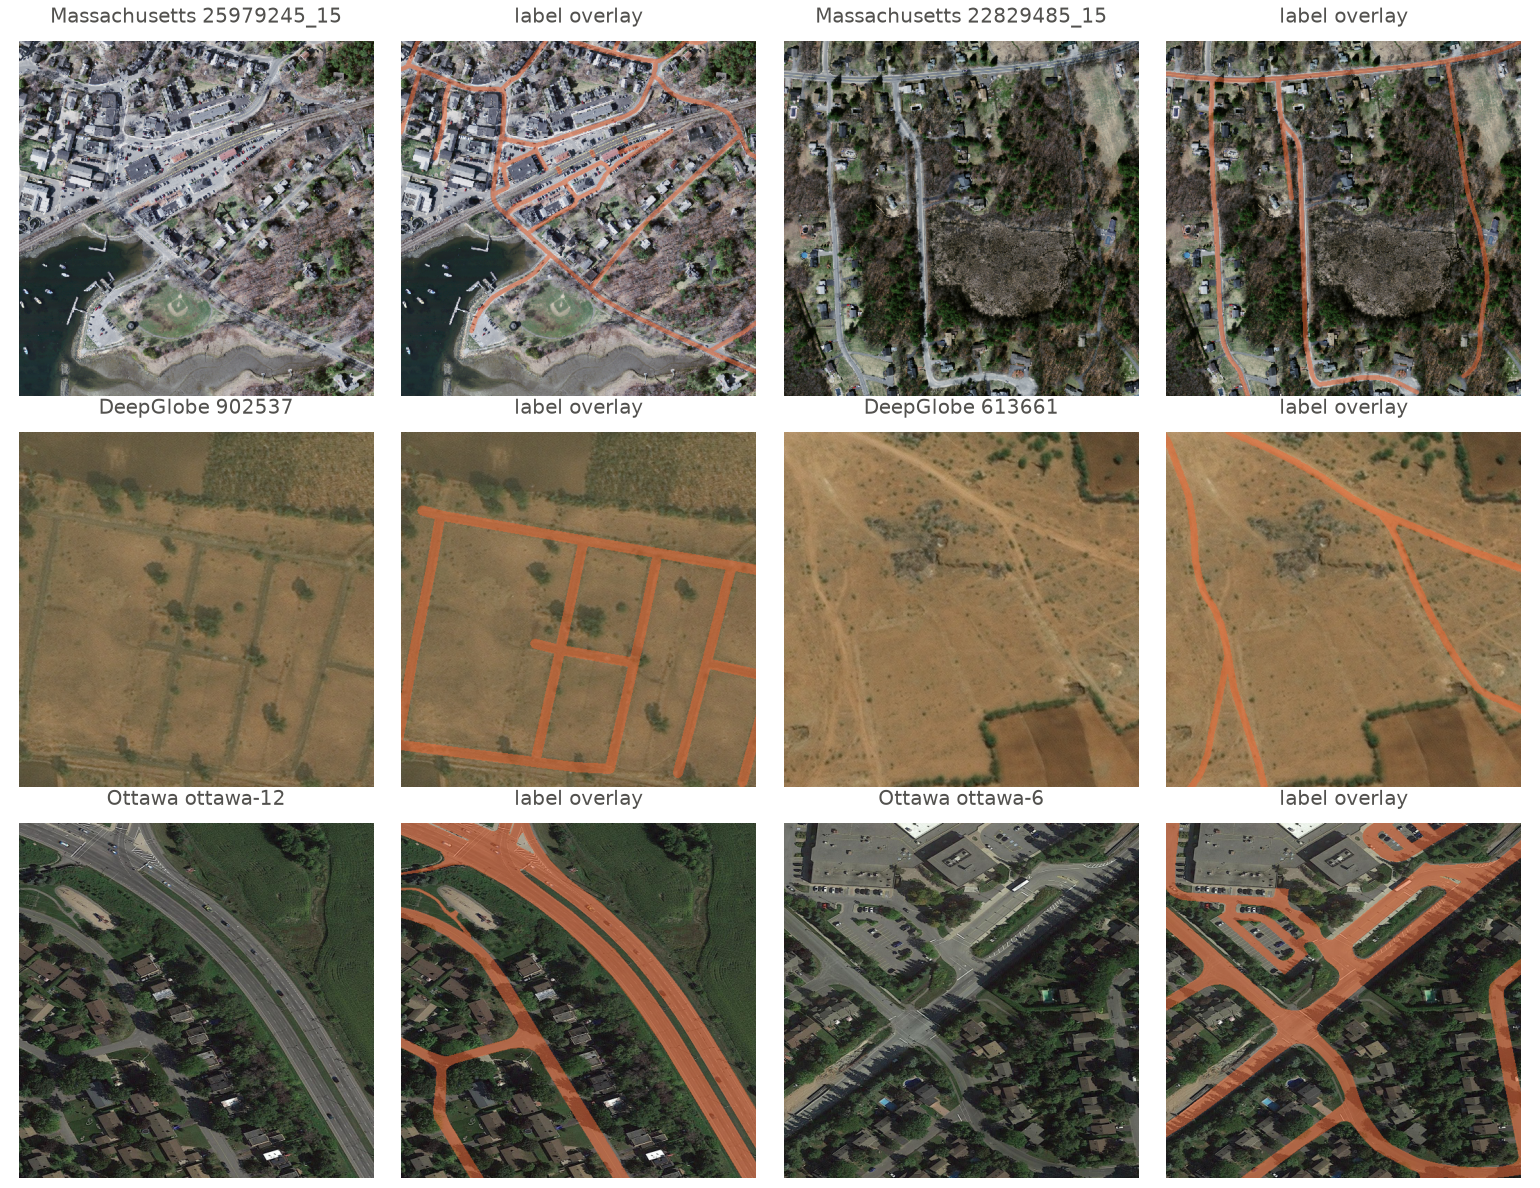
\includegraphics[width=\textwidth]{figures/datasets.png}
\caption{Training-set examples, two per dataset, each the $512\times512$ window with the most road
pixels (a fixed rule, not a hand pick); right of each image, the label overlaid in orange.
Massachusetts: fixed-width centre-line labels at 1 m. DeepGlobe: rural and peri-urban scenes at 0.5 m,
widths varying with road type. Ottawa: manually drawn road surfaces, including carriageways and
parking aisles.}
\label{fig:datasets}
\end{figure}

\begin{figure}[H]
\centering
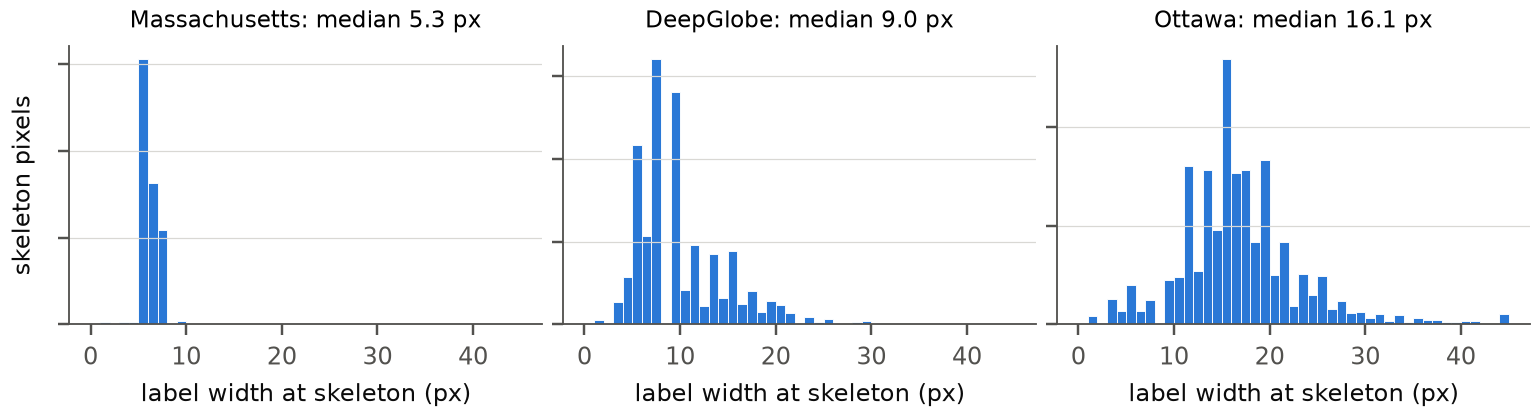
\includegraphics[width=\textwidth]{figures/widths.png}
\caption{Distribution of label width at skeleton pixels (training masks). Massachusetts: nearly
constant; DeepGlobe and Ottawa: broad.}
\label{fig:widths}
\end{figure}

\subsection{Massachusetts Roads}
Aerial RGB, 1 m/px, $1500\times1500$ tiles, labels rasterised from OpenStreetMap centre-lines
\cite{mnih2013}; official split 1108 / 14 / 49. \textbf{No-data masking}: a pixel is no-data if all
channels are $\ge 250$ and it lies in a 4-connected white region of $\ge 2500$ px (11\% of pixels on
average, up to 79\% in some tiles, with roads drawn through them). The validity mask is applied to
the loss, crop sampling, selection and every metric, so Massachusetts numbers are not directly
comparable with published ones that count those pixels.

\subsection{DeepGlobe Road Extraction}
Satellite RGB, 0.5 m/px, $1024\times1024$, Thailand/Indonesia/India \cite{demir2018}. Only the 6226
challenge training tiles have labels; they are re-split by image (seed 1337) into 4358 / 933 / 935.
Test split fingerprint (SHA-256 of sorted ids): \texttt{a18e6da5\ldots fe}. Source: HuggingFace mirror
\texttt{lammtfkday/deepglobe-roads} (counts match; pixel identity with the Kaggle release not verified).

\subsection{Ottawa (RoadNet)}
Google Earth imagery of Ottawa at 0.21 m/px with manually annotated road surfaces, edges and
centre-lines \cite{liu2019roadnet}; 20 scenes (the repository says 21). Download: authors' Google Drive
zip (SHA-256 \texttt{aacaa827\ldots 73fb6}). Preparation (\texttt{scripts/prepare\_ottawa.py}):
\begin{enumerate}
  \item Image: exact $2\times2$ box average $\to$ 0.42 m. Mask: road = green channel $<128$ (red
        labels incl.\ anti-aliased pixels), then $2\times2$ majority. Widths become 7--27 px (native
        14--54 px exceed our largest width class); the smallest scene becomes $512\times640$.
  \item Split: the authors' test scenes 1, 16--20; validation = scenes 9 and 14
        (\texttt{default\_rng(1337)} from the authors' training scenes 2--15); training = the other 12.
  \item No-imagery strips at the right edge of scenes 2 and 1 are cropped (168 and 46 columns); test
        scene 1 keeps 1.45\% black pixels (strip not a clean block). Every model is scored on the same
        pixels.
  \item Training length: 64 crops per scene per epoch (48 steps), 200 epochs (9600 steps).
\end{enumerate}

%=====================================================================================
\section{The pipeline, step by step}
\label{sec:pipeline}
%=====================================================================================

\begin{figure}[H]
\centering
\resizebox{\textwidth}{!}{%
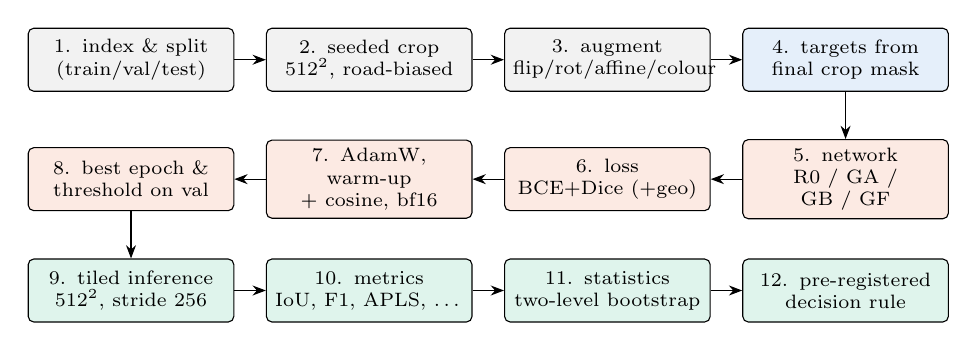
\begin{tikzpicture}[font=\scriptsize, >=Stealth, node distance=3mm and 4mm,
  b/.style={draw, rounded corners=2pt, align=center, inner sep=3pt, minimum height=8mm, text width=24mm},
  d/.style={b, fill=gray!10}, t/.style={b, fill=cblue!12}, m/.style={b, fill=corange!14}, e/.style={b, fill=caqua!14}]
\node[d] (idx) {1. index \& split\\(train/val/test)};
\node[d, right=of idx] (crop) {2. seeded crop\\$512^2$, road-biased};
\node[d, right=of crop] (aug) {3. augment\\flip/rot/affine/colour};
\node[t, right=of aug] (tgt) {4. targets from\\final crop mask};
\node[m, below=6mm of tgt] (net) {5. network\\R0 / GA / GB / GF};
\node[m, left=of net] (loss) {6. loss\\BCE+Dice (+geo)};
\node[m, left=of loss] (opt) {7. AdamW, warm-up\\+ cosine, bf16};
\node[m, left=of opt] (sel) {8. best epoch \&\\threshold on val};
\node[e, below=6mm of sel] (inf) {9. tiled inference\\$512^2$, stride 256};
\node[e, right=of inf] (met) {10. metrics\\IoU, F1, APLS, \ldots};
\node[e, right=of met] (st) {11. statistics\\two-level bootstrap};
\node[e, right=of st] (dec) {12. pre-registered\\decision rule};
\draw[->] (idx)--(crop); \draw[->] (crop)--(aug); \draw[->] (aug)--(tgt); \draw[->] (tgt)--(net);
\draw[->] (net)--(loss); \draw[->] (loss)--(opt); \draw[->] (opt)--(sel); \draw[->] (sel)--(inf);
\draw[->] (inf)--(met); \draw[->] (met)--(st); \draw[->] (st)--(dec);
\end{tikzpicture}}
\caption{End-to-end pipeline. Grey: data; blue: geometric targets; orange: model and training;
green: evaluation and inference. Steps 1--8 never open the test split.}
\label{fig:pipeline}
\end{figure}

\begin{enumerate}
  \item \textbf{Index and split.} \texttt{data/prepare.py} builds the image/mask index per dataset and
        split (Section~\ref{sec:data}); a missing mask is an error, never silently skipped. Training
        records the split sizes and, for DeepGlobe, the test fingerprint.
  \item \textbf{Seeded crops.} Each epoch draws $k\times$(number of training images) random
        $512\times512$ crops ($k=8$; Ottawa $k=64$). With probability 0.75 a crop is resampled (up to
        12 tries) until it contains road on valid pixels; crops with $<50\%$ valid pixels are
        rejected. Every crop is a pure function of (run seed, sample counter), so all models trained
        with one seed see the identical crop stream, also across preemption and resumption.
  \item \textbf{Augmentation.} Horizontal/vertical flips and $90^\circ$ rotations; with probability
        0.5 an affine warp (rotation $\pm15^\circ$, scale 0.9--1.1; bilinear image, nearest masks,
        reflective borders); with probability 0.5 brightness/contrast jitter in $[0.9,1.1]$; ImageNet
        normalisation last.
  \item \textbf{Geometric targets} (GA/GB/GAc/GAw/GF: disc cover; GD: DDT classes; GO: orientation)
        are computed from the \emph{final, augmented} crop mask in the data-loader workers
        (44--49 ms per crop). They draw no randomness, so the crop stream is R0's.
  \item \textbf{Network forward} (Section~\ref{sec:arch}) under bf16 autocast; output = mask logits at
        input resolution (asserted), plus geometric logits for the geometric models.
  \item \textbf{Loss} in fp32 (Section~\ref{sec:loss}).
  \item \textbf{Optimisation.} AdamW, $\eta_0=3\times10^{-4}$, weight decay $10^{-4}$, batch 16,
        gradient clipping at 1.0 (a non-finite loss or gradient stops the run); per-iteration
        schedule: linear warm-up from $0.01\eta_0$ over 2 epochs, then cosine to $0.01\eta_0$.
        Massachusetts 100 epochs $\times$ 554 steps; DeepGlobe 40 $\times$ 2179; Ottawa 200
        $\times$ 48. One recipe for every model.
  \item \textbf{Model and threshold selection on validation.} After each epoch, pooled validation IoU
        at threshold 0.5 on non-overlapping tiles; best epoch kept. After training, the threshold
        $\tau^\ast\in\{0.20,0.25,\dots,0.80\}$ maximising pooled validation IoU is frozen.
  \item \textbf{Tiled inference.} $512\times512$ tiles at stride 256, last row/column aligned to the
        image edge; overlapping tile probabilities averaged; $\hat Y = \{P\ge\tau^\ast\}$. The test
        split is scored exactly once per run (a second scoring is refused); probability maps are
        saved as 8-bit PNG.
  \item \textbf{Metrics} on stitched full-resolution images, valid pixels only (Section~\ref{sec:metrics}).
  \item \textbf{Statistics}: per-image paired differences, two-level bootstrap and seed-paired $t$
        (Section~\ref{sec:stats}).
  \item \textbf{Decision} by the rule written before the runs (Section~\ref{sec:prereg}).
\end{enumerate}

\paragraph{Experiment infrastructure.} Every campaign is launched by \texttt{scripts/launch.sh},
which refuses a dirty tree and requires that the CPU rehearsal passed at the same commit; it freezes
the code into \texttt{releases/<sha>/} and submits a SLURM array whose tasks import only that
snapshot. Training checkpoints atomically every 5 min and on SIGTERM/USR1, resumes exactly
(including the LR schedule and crop stream), and refuses to resume under different code. Each GPU job
first runs a 2-step self-test (preflight). A CPU rehearsal trains every model in miniature on real
data, scores, re-scores (must refuse), aggregates and runs two preemption drills. Results are
aggregated by a dependent job. The test suite has 528 tests, all passing at the final commit.

%=====================================================================================
\section{Architectures}
\label{sec:arch}
%=====================================================================================

\subsection{Shared encoder--decoder (R0)}
\textbf{Encoder}: ResNeXt-50 $32\times4$d \cite{xie2017}, ImageNet weights; each bottleneck computes
$y = x + \sum_{i=1}^{32}\mathcal{T}_i(x)$ ($1\times1$ reduce, grouped $3\times3$ with 32 groups,
$1\times1$ expand). For a $512^2$ input it emits $f_0$ (stem, $64\times256^2$), $f_1$
($256\times128^2$), $f_2$ ($512\times64^2$), $f_3$ ($1024\times32^2$), $f_4$ ($2048\times16^2$).
\textbf{Decoder}: five stages $d_\ell = \phi_\ell([\mathrm{Up}_\ell(d_{\ell-1});\,f_{4-\ell}])$,
$d_0=f_4$, with $\mathrm{Up}$ = bilinear $\times2$ + $3\times3$ conv, $\phi_\ell$ = two
Conv--BN--ReLU, widths 512, 256, 128, 64, 32 at $32^2\ldots512^2$; no skip at full resolution.
\textbf{Head}: $1\times1$ conv $\to$ one logit per pixel.

\begin{figure}[H]
\centering
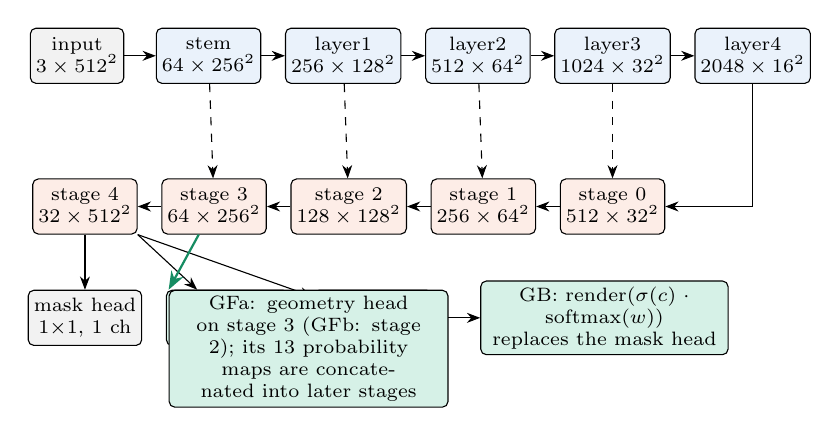
\begin{tikzpicture}[font=\scriptsize, >=Stealth,
  box/.style={draw, rounded corners=2pt, minimum height=7mm, align=center, inner sep=2pt},
  enc/.style={box, fill=cblue!10}, dec/.style={box, fill=corange!12}, op/.style={box, fill=gray!10},
  geo/.style={box, fill=caqua!18}]
\node[op] (in) {input\\$3\times512^2$};
\node[enc, right=4mm of in] (stem) {stem\\$64\times256^2$};
\node[enc, right=3mm of stem] (l1) {layer1\\$256\times128^2$};
\node[enc, right=3mm of l1] (l2) {layer2\\$512\times64^2$};
\node[enc, right=3mm of l2] (l3) {layer3\\$1024\times32^2$};
\node[enc, right=3mm of l3] (l4) {layer4\\$2048\times16^2$};
\foreach \a/\b in {in/stem,stem/l1,l1/l2,l2/l3,l3/l4} \draw[->] (\a)--(\b);
\node[dec, below=12mm of l3] (d1) {stage 0\\$512\times32^2$};
\node[dec, left=3mm of d1] (d2) {stage 1\\$256\times64^2$};
\node[dec, left=3mm of d2] (d3) {stage 2\\$128\times128^2$};
\node[dec, left=3mm of d3] (d4) {stage 3\\$64\times256^2$};
\node[dec, left=3mm of d4] (d5) {stage 4\\$32\times512^2$};
\draw[->] (l4) |- (d1); \foreach \a/\b in {d1/d2,d2/d3,d3/d4,d4/d5} \draw[->] (\a)--(\b);
\draw[->, dashed] (l3)--(d1); \draw[->, dashed] (l2)--(d2); \draw[->, dashed] (l1)--(d3); \draw[->, dashed] (stem)--(d4);
\node[op, below=7mm of d5] (mh) {mask head\\$1{\times}1$, 1 ch};
\node[geo, right=3mm of mh] (ch) {centre head\\$1{\times}1$, 1 ch};
\node[geo, right=3mm of ch] (wh) {width head\\$1{\times}1$, 12 ch};
\node[geo, right=6mm of wh, text width=30mm] (rd) {GB: $\mathrm{render}(\sigma(c)\cdot\mathrm{softmax}(w))$\\replaces the mask head};
\draw[->] (d5)--(mh); \draw[->] (d5.south east) -- (ch); \draw[->] (d5.south east) -- (wh); \draw[->] (wh)--(rd);
\node[geo, below=7mm of d4, xshift=12mm, text width=34mm] (gf) {GFa: geometry head on stage 3 (GFb: stage 2); its 13 probability maps are concatenated into later stages};
\draw[->, caqua!80!black, thick] (d4) -- (gf.north west);
\end{tikzpicture}
\caption{Shared ResNeXt-50 U-Net (R0) and the geometric variants. Dashed: skip connections. GA adds the
two green heads on the 32-channel full-resolution features as auxiliary outputs (discarded at
inference); GB draws the mask from them; GF moves the geometry head into the decoder and feeds its
output back.}
\label{fig:arch}
\end{figure}

\subsection{GA: geometric auxiliary heads}
Two $1\times1$ convolutions on the final 32-channel feature map: a centre-line logit $c$ and 12
width-class logits $w$ (radii $\mathcal R = \{0,1,2,3,4,5,6,8,10,13,16,20\}$ px). The mask comes from
R0's own head; the geometric heads only add training signal and are not used at inference
($+429$ parameters, identical inference cost). Built after R0's modules, so at a given seed every
shared weight is bitwise identical to R0's.

\subsection{GB: the mask drawn from centre and width}
GB uses the same heads but its mask is $m = \mathrm{render}(\sigma(c)\odot\mathrm{softmax}(w))$:
each candidate centre pixel is dilated by its radius class, with an octagonal disc that is the
Minkowski sum of alternating $3\times3$ square/cross steps.
\begin{algorithm}[H]
\caption{\texttt{render}: variable-radius dilation in one pass of max-pools}
\begin{algorithmic}[1]
\Require contributions $q_k = \sigma(c)\,\mathrm{softmax}(w)_k$ for radii $r_k\in\mathcal R$
\State $o \gets$ none
\For{$j = \max\mathcal R$ \textbf{down to} $0$}
  \For{each $k$ with $r_k = j$} \State $o \gets \max(o, q_k)$ \EndFor
  \If{$j>0$} \State $o \gets \mathrm{maxpool}_{3\times3}(o)$ if $j$ odd, else cross-shaped max-pool \EndIf
\EndFor
\State \Return $o$ \Comment{each bin dilated by exactly its radius; differentiable; 20 max-pools}
\end{algorithmic}
\end{algorithm}
The logit $\log m - \log(1-m)$ (with $m$ clamped to $[10^{-4},1-10^{-4}]$) is returned so thresholding,
inference and scoring are R0's code unchanged. R0's mask head is kept but unused.

\subsection{GF: geometry fed back into the decoder}
A $1\times1$ geometry head (13 channels: 1 centre + 12 width) is applied after decoder stage 3
($64\times256^2$, GFa) or stage 2 ($128\times128^2$, GFb). Its probabilities
$[\sigma(c);\mathrm{softmax}(w)]$ are bilinearly resized and concatenated into the input of every later
stage, whose first convolution gains 13 input channels. The geometric logits are upsampled to full
resolution for the loss. Tests confirm that changing only the geometry head changes the mask, and that
the mask loss alone trains the geometry head. Parameters: $+4{,}589$ (GFa), $+12{,}909$ (GFb).

\subsection{Baselines on the same model}
\begin{itemize}
  \item \textbf{GAc / GAw}: GA with the width (GAc) or the centre (GAw) loss weight set to 0.
  \item \textbf{GD}: Deep Distance Transform targets \cite{wang2020ddt}: at every road pixel,
        $\mathrm{round}(\EDT)$ as one of 20 classes; no centre term ($+693$ parameters).
  \item \textbf{GO}: orientation \cite{batra2019}: the undirected direction of the nearest
        skeleton segment (structure tensor of the blurred skeleton) in 18 bins of $10^\circ$ plus a
        background class, supervised at every pixel ($+660$ parameters).
  \item \textbf{Paper-1 models} (appendix): R1--R3 (wavelets), U-Net from scratch, D-LinkNet.
\end{itemize}

\begin{table}[H]
\centering
\caption{Trainable parameters.}
\small
\begin{tabular}{@{}lrr@{}}
\toprule
Model & Parameters & vs.\ R0 \\
\midrule
R0 & 46{,}503{,}137 & --- \\
GA, GB, GAc, GAw & 46{,}503{,}566 & $+429$ \\
GD & 46{,}503{,}830 & $+693$ \\
GO & 46{,}503{,}797 & $+660$ \\
GFa & 46{,}507{,}726 & $+4{,}589$ \\
GFb & 46{,}516{,}046 & $+12{,}909$ \\
U-Net (scratch) / D-LinkNet & 31{,}037{,}633 / 31{,}095{,}137 & --- \\
\bottomrule
\end{tabular}
\end{table}

%=====================================================================================
\section{Geometric targets}
\label{sec:targets}
%=====================================================================================

Let $M$ be the binary mask of a training crop.
\begin{enumerate}
  \item \textbf{Padding.} $M$ is padded by edge replication (21 px) so a road leaving the crop is not
        treated as ending there; results are cropped back.
  \item \textbf{Disc depth.} For radius $r$, the disc $D_r$ is the Minkowski sum of the steps
        $j=r,\dots,1$ (square for odd $j$, cross for even $j$) --- exactly the shape \texttt{render}
        draws. With $E_0=M$ and $E_j = E_{j-1}\ominus \mathrm{step}(j)$, $E_r = M\ominus D_r$; the depth
        of a pixel is the largest $r\in\mathcal R$ with the pixel in $E_r$.
  \item \textbf{Centre pixels} $S$: $\mathrm{skeletonize}(M)$, then every mask pixel not covered by
        $\bigcup_{p\in S} (p + D_{\mathrm{depth}(p)})$ is added with its own depth (after cropping).
  \item \textbf{Targets}: centre map $=\mathbf 1_S$; width class = depth at $S$, ignored elsewhere and
        on no-data pixels.
\end{enumerate}
\begin{proposition}[Exactness]
Every disc lies inside $M$ (by the definition of depth) and every pixel of $M$ is covered (by step 3),
so $\mathrm{render}$ of the one-hot targets equals $M$.
\end{proposition}
Measured on 60 training images per dataset: drawn-back IoU $1.000000$ (worst image $1.000000$) on full
images and $512^2$ crops. The skeleton alone would reach 0.8817 (Massachusetts) / 0.9177 (DeepGlobe);
about half the centre pixels are skeleton, the rest are 1-px staircase edge pixels with radius 0--1.
Design history (training masks only): skeleton + nearest radius to $\EDT - o$ reached 0.806 / 0.910 /
0.881 for $o = 0.5 / 1.0 / 1.5$ (Massachusetts); adding equal-depth neighbours for even widths did not
help (0.910); diagnosis showed every error to be a 1-px edge pixel on slanted roads.

\begin{figure}[H]
\centering
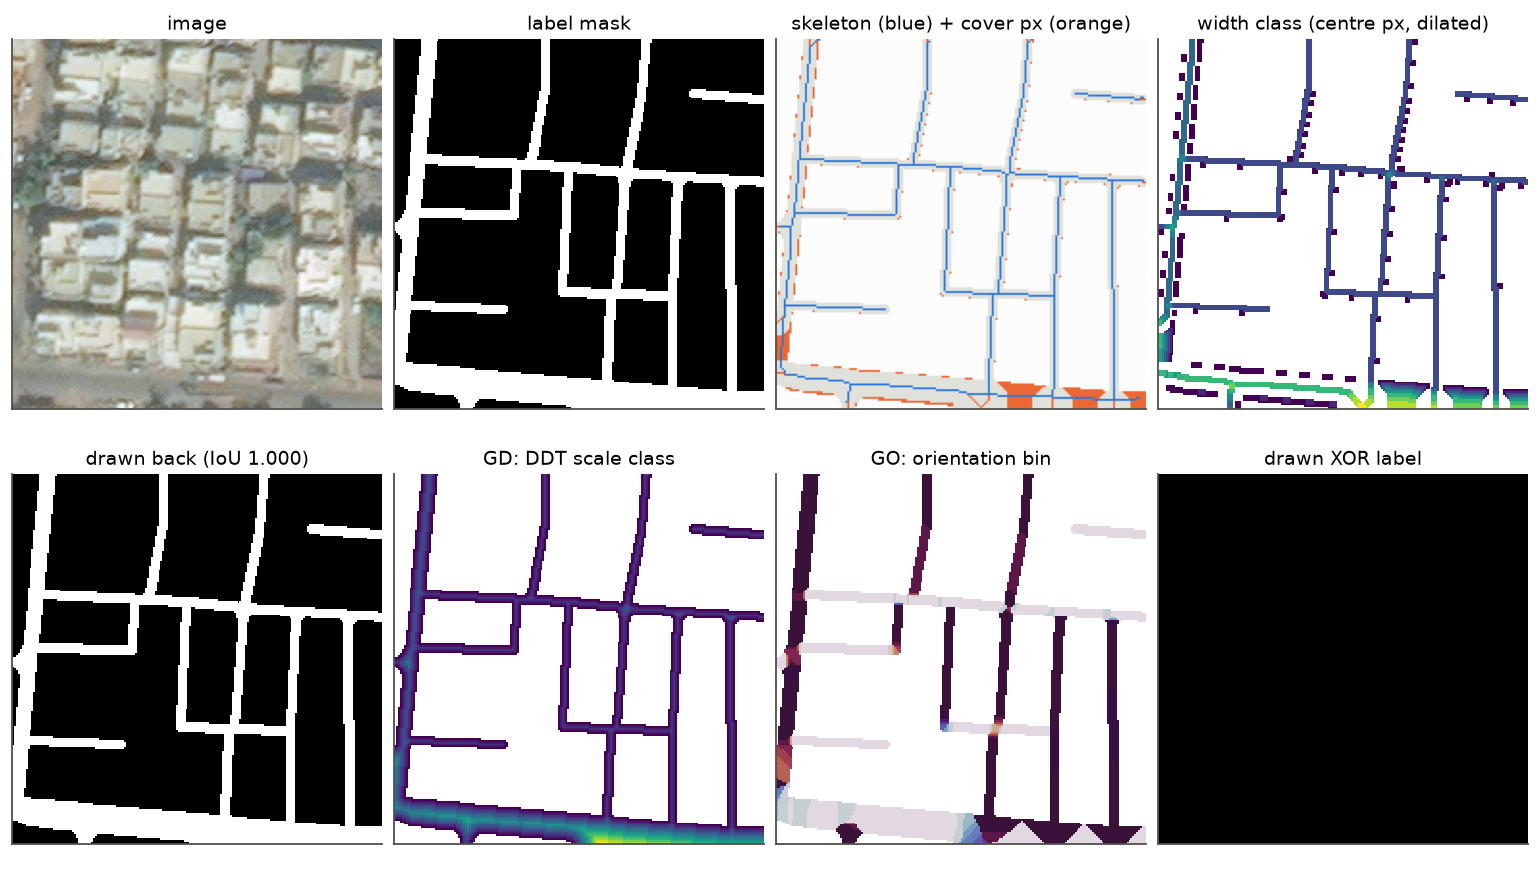
\includegraphics[width=\textwidth]{figures/targets.png}
\caption{Targets on a DeepGlobe training crop (the $192^2$ window with the most skeleton junctions).
Top: image, label, skeleton (blue) and added cover pixels (orange), width class at centre pixels.
Bottom: the label drawn back from the targets (exact), DDT scale classes (GD), orientation bins (GO),
and the XOR of drawn-back and label (empty).}
\label{fig:targets}
\end{figure}

%=====================================================================================
\section{Loss functions}
\label{sec:loss}
%=====================================================================================

With logits $z$, $p=\sigma(z)$, label $y$ and validity $v$:
\begin{align}
\mathcal L_{\mathrm{BCE}}(z,y) &= \frac{\sum v\,\mathrm{bce}(z,y)}{\max(\sum v,1)}, \qquad
\mathcal L_{\mathrm{Dice}}(z,y) = 1 - \frac{2\sum p\,y\,v + 1}{\sum p\,v + \sum y\,v + 1},\\
\mathcal L_{\mathrm{R0}} &= \mathcal L_{\mathrm{BCE}}(z_m,y) + \mathcal L_{\mathrm{Dice}}(z_m,y),\\
\mathcal L_{\mathrm{geo}} &= \mathcal L_{\mathrm{R0}} + \lambda_c\big[\mathcal L_{\mathrm{BCE}}(z_c,\mathbf 1_S)+\mathcal L_{\mathrm{Dice}}(z_c,\mathbf 1_S)\big]
  + \lambda_w\,\frac{1}{|S_v|}\sum_{u\in S_v}\mathrm{CE}\big(z_w(u),\,k(u)\big),
\end{align}
with $\lambda_c=\lambda_w=1$ (untuned) for GA/GB/GF, $(1,0)$ for GAc, $(0,1)$ for GAw; for GD and GO the
class term runs over road pixels (GD) or all valid pixels (GO) and $\lambda_c=0$. For GB, $z_m$ is the
logit of the drawn mask. All losses in fp32; Dice smoothing 1 keeps road-free crops stable.

%=====================================================================================
\section{Metrics}
\label{sec:metrics}
%=====================================================================================

Counts TP, FP, FN, TN over valid pixels of stitched test images at $\tau^\ast$.
\begin{itemize}
  \item \textbf{IoU} (road) $=\frac{TP}{TP+FP+FN}$, pooled (counts summed over images) and per image
        (IoU$_{img}$, the unit of the statistics).
  \item \textbf{mIoU} $=\frac12\big(\frac{TP}{TP+FP+FN}+\frac{TN}{TN+FP+FN}\big)$.
  \item \textbf{F1} $=\frac{2TP}{2TP+FP+FN}$, \textbf{precision} $=\frac{TP}{TP+FP}$,
        \textbf{recall} $=\frac{TP}{TP+FN}$, \textbf{accuracy} $=\frac{TP+TN}{TP+TN+FP+FN}$ (pooled).
  \item \textbf{Relaxed F1} ($\rho=3$ px) \cite{mnih2010}, \textbf{clDice} \cite{shit2021},
        \textbf{APLS} \cite{vanetten2018} (graphs from skeletons, 500 node pairs per direction, 8 px
        snapping, a missing node scores 0), all per image then averaged.
\end{itemize}
Accuracy is dominated by background (roads are 4--15\% of pixels) and is reported for completeness.

%=====================================================================================
\section{Statistical analysis}
\label{sec:stats}
%=====================================================================================

For arms $a\in\{0,1\}$, seeds $s$ and images $i=1..N$, $\hat\Delta = \frac1N\sum_i(\bar u_{1,i}-\bar u_{0,i})$.
\textbf{Two-level bootstrap} ($B=10{,}000$, seed 0): resample seeds within each arm, then images
(paired), percentile interval. \textbf{Seed-paired $t$}: $d_s=\frac1N\sum_i(u_{1,s,i}-u_{0,s,i})$ over
common seeds, $\bar d\pm t_{0.975,n-1}s_d/\sqrt n$. \textbf{Decision rule}: \emph{difference} if both
intervals exclude zero with the same sign; \emph{inconclusive} if exactly one does; \emph{no detected
difference} if neither. With 3 seeds the bootstrap can be anti-conservative (simulated coverage
0.86--0.98), hence the second interval. Secondary analyses carry no multiplicity correction and are
labelled as such.

\subsection{Pre-registration}
\label{sec:prereg}
\begin{table}[H]
\centering
\caption{Analysis plans (\texttt{src/roadseg/stats.py}) and when they were fixed.}
\small
\begin{tabular}{@{}p{1.4cm}p{3.6cm}p{5.4cm}p{3.6cm}@{}}
\toprule
Plan & Primary & Fixed & Commit \\
\midrule
\texttt{geo} & GB $-$ R0 (each dataset) & before any GA/GB run & ffe5351 \\
(ledger) & GA $-$ R0, DeepGlobe & 2026-10-15 13:29, before the DeepGlobe result was read & e48f87c \\
\texttt{geo2} & GA $-$ R0, Massachusetts, 5 seeds & before any geo2 run & a6cc48b \\
\texttt{geo3} & GA $-$ GD, DeepGlobe & before any GD/GO run & ba1e8e9 \\
\texttt{ott} & GA $-$ R0, Ottawa, 5 seeds & before any Ottawa run & 8cb06c4 \\
\texttt{gf\_a/b} & GF $-$ R0 (each dataset); variant chosen on validation & before any GF run & c430651 \\
\bottomrule
\end{tabular}
\end{table}

%=====================================================================================
\section{Results}
\label{sec:results}
%=====================================================================================

\subsection{All metrics}
\begin{table}[H]
\centering
\caption{Test metrics, mean over $n$ seeds; best per dataset in bold. Pooled metrics except IoU$_{img}$,
F1$_{\rho=3}$, clDice and APLS (per-image means). $^\dagger$Paper-1 models. GFb is the single
selection run (seed 0), shown for completeness.}
\label{tab:all}
\scriptsize
\setlength{\tabcolsep}{3pt}
\resizebox{\textwidth}{!}{\begin{tabular}{@{}lrrrrrrrrrrr@{}}
\toprule
Model & $n$ & IoU & mIoU & F1 & Prec. & Rec. & Acc. & IoU$_{img}$ & F1$_{\rho=3}$ & clDice & APLS \\
\midrule
\multicolumn{12}{@{}l}{\textbf{Massachusetts}} \\
R0 (ResNeXt-50 U-Net) & 5 & 0.6556 & 0.8177 & 0.7920 & 0.7979 & 0.7862 & 0.9806 & 0.6519 & 0.9065 & 0.8804 & 0.8007 \\
R1 (DWT input)$^{\dagger}$ & 3 & 0.6554 & 0.8176 & 0.7918 & 0.7967 & 0.7871 & 0.9805 & 0.6533 & 0.9087 & 0.8821 & 0.8029 \\
R2 (wavelet pool)$^{\dagger}$ & 3 & 0.6545 & 0.8170 & 0.7912 & 0.7900 & 0.7924 & 0.9803 & 0.6520 & 0.9079 & 0.8822 & 0.8029 \\
R3 (R2 + clDice)$^{\dagger}$ & 3 & 0.6553 & 0.8175 & 0.7918 & 0.7898 & 0.7937 & 0.9804 & 0.6511 & 0.9060 & 0.8828 & \textbf{0.8040} \\
U-Net (scratch)$^{\dagger}$ & 3 & \textbf{0.6632} & \textbf{0.8217} & \textbf{0.7975} & 0.7961 & \textbf{0.7989} & \textbf{0.9809} & \textbf{0.6624} & \textbf{0.9155} & \textbf{0.8895} & 0.8006 \\
D-LinkNet$^{\dagger}$ & 3 & 0.6515 & 0.8154 & 0.7890 & 0.7895 & 0.7884 & 0.9802 & 0.6486 & 0.9080 & 0.8806 & 0.8002 \\
GA (aux. centre+width) & 5 & 0.6588 & 0.8194 & 0.7943 & 0.8031 & 0.7856 & 0.9809 & 0.6546 & 0.9077 & 0.8822 & 0.8029 \\
GB (drawn mask) & 3 & 0.6555 & 0.8176 & 0.7919 & 0.7929 & 0.7909 & 0.9805 & 0.6508 & 0.9054 & 0.8831 & 0.7990 \\
GFa (geometry feedback) & 3 & 0.6591 & 0.8196 & 0.7945 & \textbf{0.8051} & 0.7842 & \textbf{0.9809} & 0.6552 & 0.9071 & 0.8832 & 0.8008 \\
GFb (feedback, 1/4) & 1 & 0.6584 & 0.8192 & 0.7940 & 0.8022 & 0.7859 & 0.9808 & 0.6548 & 0.9072 & 0.8839 & 0.8015 \\
\midrule
\multicolumn{12}{@{}l}{\textbf{DeepGlobe}} \\
R0 (ResNeXt-50 U-Net) & 3 & 0.6771 & 0.8306 & 0.8074 & 0.7976 & 0.8175 & 0.9846 & 0.6751 & 0.8978 & 0.8665 & 0.7755 \\
R1 (DWT input)$^{\dagger}$ & 3 & 0.6785 & 0.8314 & 0.8085 & 0.8005 & 0.8167 & 0.9847 & 0.6768 & 0.8988 & 0.8670 & 0.7777 \\
R2 (wavelet pool)$^{\dagger}$ & 3 & 0.6823 & 0.8333 & 0.8111 & 0.8008 & 0.8217 & 0.9848 & 0.6790 & 0.8996 & \textbf{0.8687} & \textbf{0.7814} \\
R3 (R2 + clDice)$^{\dagger}$ & 3 & 0.6743 & 0.8291 & 0.8054 & 0.7959 & 0.8153 & 0.9844 & 0.6723 & 0.8952 & 0.8683 & 0.7763 \\
U-Net (scratch)$^{\dagger}$ & 3 & 0.6461 & 0.8141 & 0.7850 & 0.7745 & 0.7958 & 0.9827 & 0.6419 & 0.8764 & 0.8378 & 0.7193 \\
D-LinkNet$^{\dagger}$ & 3 & 0.6655 & 0.8245 & 0.7992 & 0.7932 & 0.8053 & 0.9840 & 0.6669 & 0.8955 & 0.8613 & 0.7614 \\
GA (aux. centre+width) & 3 & \textbf{0.6858} & \textbf{0.8352} & \textbf{0.8136} & \textbf{0.8087} & 0.8186 & \textbf{0.9851} & 0.6824 & 0.8985 & 0.8659 & 0.7753 \\
GB (drawn mask) & 3 & 0.6781 & 0.8311 & 0.8082 & 0.7944 & \textbf{0.8225} & 0.9845 & 0.6733 & 0.8940 & 0.8680 & 0.7588 \\
GAc (centre only) & 3 & 0.6784 & 0.8313 & 0.8084 & 0.8018 & 0.8150 & 0.9847 & 0.6755 & 0.8976 & 0.8661 & 0.7759 \\
GAw (width only) & 3 & 0.6849 & 0.8347 & 0.8130 & 0.8069 & 0.8193 & 0.9851 & 0.6793 & 0.8962 & 0.8639 & 0.7748 \\
GD (DDT targets) & 3 & 0.6834 & 0.8339 & 0.8119 & 0.8055 & 0.8184 & 0.9850 & 0.6777 & 0.8954 & 0.8615 & 0.7717 \\
GO (orientation) & 3 & 0.6812 & 0.8328 & 0.8104 & 0.8039 & 0.8170 & 0.9849 & 0.6764 & 0.8982 & 0.8667 & 0.7768 \\
GFa (geometry feedback) & 3 & 0.6850 & 0.8348 & 0.8131 & 0.8077 & 0.8185 & 0.9851 & 0.6806 & 0.8968 & 0.8651 & 0.7745 \\
GFb (feedback, 1/4) & 1 & 0.6857 & 0.8352 & 0.8136 & 0.8085 & 0.8187 & \textbf{0.9851} & \textbf{0.6830} & \textbf{0.9002} & 0.8682 & 0.7805 \\
\midrule
\multicolumn{12}{@{}l}{\textbf{Ottawa}} \\
R0 (ResNeXt-50 U-Net) & 5 & \textbf{0.8861} & \textbf{0.9342} & \textbf{0.9396} & 0.9327 & \textbf{0.9466} & \textbf{0.9843} & \textbf{0.8798} & \textbf{0.9783} & \textbf{0.9609} & \textbf{0.8828} \\
GA (aux. centre+width) & 5 & 0.8828 & 0.9322 & 0.9377 & 0.9359 & 0.9396 & 0.9839 & 0.8769 & 0.9760 & 0.9542 & 0.8394 \\
GD (DDT targets) & 5 & 0.8808 & 0.9312 & 0.9366 & \textbf{0.9396} & 0.9337 & 0.9837 & 0.8750 & 0.9749 & 0.9545 & 0.8198 \\
GFa (geometry feedback) & 3 & 0.8833 & 0.9326 & 0.9381 & 0.9366 & 0.9396 & 0.9840 & 0.8766 & 0.9765 & 0.9569 & 0.8644 \\
GFb (feedback, 1/4) & 1 & 0.8824 & 0.9321 & 0.9375 & 0.9386 & 0.9365 & 0.9839 & 0.8768 & 0.9758 & 0.9585 & 0.8744 \\
\bottomrule
\end{tabular}
}
\end{table}

\begin{table}[H]
\centering
\caption{Pooled test IoU and F1 with seed standard deviation, validation IoU at the selected threshold,
selected threshold and training time (GPU-hours per run, NVIDIA L40S).}
\scriptsize
\resizebox{\textwidth}{!}{\begin{tabular}{@{}llrrrrr@{}}
\toprule
Model & seeds & test IoU & test F1 & val IoU & thr. & GPU-h \\
\midrule
\multicolumn{7}{@{}l}{\textbf{Massachusetts}} \\
R0 (ResNeXt-50 U-Net) & 0,1,2,3,4 & 0.6556\,$\pm$\,0.0018 & 0.7920\,$\pm$\,0.0013 & 0.6470\,$\pm$\,0.0017 & 0.40 & 3.7 \\
R1 (DWT input) & 0,1,2 & 0.6554\,$\pm$\,0.0024 & 0.7918\,$\pm$\,0.0018 & 0.6470\,$\pm$\,0.0004 & 0.40 & 3.7 \\
R2 (wavelet pool) & 0,1,2 & 0.6545\,$\pm$\,0.0001 & 0.7912\,$\pm$\,0.0001 & 0.6458\,$\pm$\,0.0025 & 0.37 & 3.8 \\
R3 (R2 + clDice) & 0,1,2 & 0.6553\,$\pm$\,0.0018 & 0.7918\,$\pm$\,0.0013 & 0.6449\,$\pm$\,0.0026 & 0.43 & 3.9 \\
U-Net (scratch) & 0,1,2 & 0.6632\,$\pm$\,0.0001 & 0.7975\,$\pm$\,0.0001 & 0.6514\,$\pm$\,0.0020 & 0.35 & 5.0 \\
D-LinkNet & 0,1,2 & 0.6515\,$\pm$\,0.0014 & 0.7890\,$\pm$\,0.0010 & 0.6391\,$\pm$\,0.0014 & 0.38 & 1.2 \\
GA (aux. centre+width) & 0,1,2,3,4 & 0.6588\,$\pm$\,0.0008 & 0.7943\,$\pm$\,0.0006 & 0.6495\,$\pm$\,0.0013 & 0.43 & 3.9 \\
GB (drawn mask) & 0,1,2 & 0.6555\,$\pm$\,0.0004 & 0.7919\,$\pm$\,0.0003 & 0.6462\,$\pm$\,0.0008 & 0.35 & 4.4 \\
GFa (geometry feedback) & 0,1,2 & 0.6591\,$\pm$\,0.0018 & 0.7945\,$\pm$\,0.0013 & 0.6488\,$\pm$\,0.0024 & 0.40 & 4.2 \\
GFb (feedback, 1/4) & 0 & 0.6584 & 0.7940 & 0.6498 & 0.40 & 4.4 \\
\midrule
\multicolumn{7}{@{}l}{\textbf{DeepGlobe}} \\
R0 (ResNeXt-50 U-Net) & 0,1,2 & 0.6771\,$\pm$\,0.0023 & 0.8074\,$\pm$\,0.0016 & 0.6806\,$\pm$\,0.0025 & 0.45 & 6.1 \\
R1 (DWT input) & 0,1,2 & 0.6785\,$\pm$\,0.0010 & 0.8085\,$\pm$\,0.0007 & 0.6805\,$\pm$\,0.0011 & 0.45 & 6.1 \\
R2 (wavelet pool) & 0,1,2 & 0.6823\,$\pm$\,0.0011 & 0.8111\,$\pm$\,0.0008 & 0.6839\,$\pm$\,0.0016 & 0.45 & 6.4 \\
R3 (R2 + clDice) & 0,1,2 & 0.6743\,$\pm$\,0.0013 & 0.8054\,$\pm$\,0.0009 & 0.6775\,$\pm$\,0.0002 & 0.48 & 6.5 \\
U-Net (scratch) & 0,1,2 & 0.6461\,$\pm$\,0.0008 & 0.7850\,$\pm$\,0.0006 & 0.6512\,$\pm$\,0.0005 & 0.45 & 8.1 \\
D-LinkNet & 0,1,2 & 0.6655\,$\pm$\,0.0005 & 0.7992\,$\pm$\,0.0004 & 0.6687\,$\pm$\,0.0003 & 0.48 & 2.1 \\
GA (aux. centre+width) & 0,1,2 & 0.6858\,$\pm$\,0.0007 & 0.8136\,$\pm$\,0.0005 & 0.6885\,$\pm$\,0.0005 & 0.45 & 6.5 \\
GB (drawn mask) & 0,1,2 & 0.6781\,$\pm$\,0.0008 & 0.8082\,$\pm$\,0.0006 & 0.6813\,$\pm$\,0.0003 & 0.38 & 7.2 \\
GAc (centre only) & 0,1,2 & 0.6784\,$\pm$\,0.0008 & 0.8084\,$\pm$\,0.0006 & 0.6808\,$\pm$\,0.0011 & 0.45 & 6.5 \\
GAw (width only) & 0,1,2 & 0.6849\,$\pm$\,0.0004 & 0.8130\,$\pm$\,0.0003 & 0.6887\,$\pm$\,0.0009 & 0.45 & 6.5 \\
GD (DDT targets) & 0,1,2 & 0.6834\,$\pm$\,0.0006 & 0.8119\,$\pm$\,0.0004 & 0.6870\,$\pm$\,0.0008 & 0.45 & 6.7 \\
GO (orientation) & 0,1,2 & 0.6812\,$\pm$\,0.0029 & 0.8104\,$\pm$\,0.0020 & 0.6849\,$\pm$\,0.0023 & 0.47 & 6.6 \\
GFa (geometry feedback) & 0,1,2 & 0.6850\,$\pm$\,0.0018 & 0.8131\,$\pm$\,0.0012 & 0.6881\,$\pm$\,0.0003 & 0.45 & 7.0 \\
GFb (feedback, 1/4) & 0 & 0.6857 & 0.8136 & 0.6890 & 0.45 & 7.0 \\
\midrule
\multicolumn{7}{@{}l}{\textbf{Ottawa}} \\
R0 (ResNeXt-50 U-Net) & 0,1,2,3,4 & 0.8861\,$\pm$\,0.0048 & 0.9396\,$\pm$\,0.0027 & 0.9015\,$\pm$\,0.0009 & 0.48 & 0.7 \\
GA (aux. centre+width) & 0,1,2,3,4 & 0.8828\,$\pm$\,0.0036 & 0.9377\,$\pm$\,0.0020 & 0.8922\,$\pm$\,0.0027 & 0.52 & 0.9 \\
GD (DDT targets) & 0,1,2,3,4 & 0.8808\,$\pm$\,0.0023 & 0.9366\,$\pm$\,0.0013 & 0.8935\,$\pm$\,0.0027 & 0.58 & 0.8 \\
GFa (geometry feedback) & 0,1,2 & 0.8833\,$\pm$\,0.0024 & 0.9381\,$\pm$\,0.0014 & 0.8981\,$\pm$\,0.0024 & 0.43 & 0.9 \\
GFb (feedback, 1/4) & 0 & 0.8824 & 0.9375 & 0.8986 & 0.65 & 0.9 \\
\bottomrule
\end{tabular}
}
\end{table}

\subsection{Pre-specified and secondary comparisons}
\begin{table}[H]
\centering
\caption{All comparisons. $n_s$ = seeds of the first arm. Two intervals as in Section~\ref{sec:stats}.}
\label{tab:cmp}
\scriptsize
\setlength{\tabcolsep}{3pt}
\resizebox{\textwidth}{!}{\begin{tabular}{@{}lrrllrll@{}}
\toprule
Comparison & $n_s$ & $\hat\Delta$ IoU$_{img}$ & two-level 95\% CI & seed-paired $t$ 95\% CI & $\Delta$ pooled & decision & role \\
\midrule
\multicolumn{8}{@{}l}{\textbf{Massachusetts}} \\
GB -- R0 & 3 & -0.0012 & [-0.0050, +0.0027] & [-0.0056, +0.0013] & -0.0002 & no detected diff. & primary (geo) \\
GA -- R0 & 5 & +0.0027 & [-0.0012, +0.0068] & [-0.0008, +0.0061] & +0.0031 & no detected diff. & primary (geo2, 5 seeds) \\
GFa -- R0 & 3 & +0.0032 & [-0.0018, +0.0085] & [-0.0031, +0.0077] & +0.0035 & no detected diff. & primary (gf\_a) \\
GB -- GA & 3 & -0.0038 & [-0.0078, -0.0002] & [-0.0083, -0.0008] & -0.0033 & difference & secondary \\
GFa -- GA & 3 & +0.0006 & [-0.0038, +0.0047] & [-0.0062, +0.0059] & +0.0003 & no detected diff. & secondary \\
\midrule
\multicolumn{8}{@{}l}{\textbf{DeepGlobe}} \\
GB -- R0 & 3 & -0.0017 & [-0.0059, +0.0028] & [-0.0129, +0.0095] & +0.0011 & no detected diff. & primary (geo) \\
GA -- R0 & 3 & +0.0073 & [+0.0033, +0.0118] & [+0.0011, +0.0135] & +0.0087 & difference & confirmatory (registered 13:29, 15 Oct) \\
GAc -- R0 & 3 & +0.0005 & [-0.0033, +0.0051] & [-0.0098, +0.0108] & +0.0013 & no detected diff. & secondary \\
GAw -- R0 & 3 & +0.0043 & [+0.0002, +0.0088] & [-0.0013, +0.0098] & +0.0078 & inconclusive & secondary \\
GD -- R0 & 3 & +0.0027 & [-0.0012, +0.0070] & [-0.0048, +0.0101] & +0.0063 & no detected diff. & secondary \\
GO -- R0 & 3 & +0.0014 & [-0.0041, +0.0068] & [-0.0147, +0.0175] & +0.0041 & no detected diff. & secondary \\
GFa -- R0 & 3 & +0.0056 & [+0.0012, +0.0103] & [-0.0072, +0.0183] & +0.0080 & inconclusive & primary (gf\_a) \\
GB -- GA & 3 & -0.0090 & [-0.0118, -0.0062] & [-0.0155, -0.0025] & -0.0077 & difference & secondary \\
GFa -- GA & 3 & -0.0017 & [-0.0048, +0.0013] & [-0.0083, +0.0048] & -0.0008 & no detected diff. & secondary \\
GD -- GA & 3 & -0.0046 & [-0.0072, -0.0022] & [-0.0068, -0.0025] & -0.0024 & difference & secondary \\
GO -- GA & 3 & -0.0059 & [-0.0110, -0.0017] & [-0.0161, +0.0042] & -0.0046 & inconclusive & secondary \\
GAc -- GA & 3 & -0.0068 & [-0.0101, -0.0035] & [-0.0111, -0.0025] & -0.0074 & difference & secondary \\
GAw -- GA & 3 & -0.0030 & [-0.0057, -0.0004] & [-0.0042, -0.0019] & -0.0009 & difference & secondary \\
GA -- GD & 3 & +0.0046 & [+0.0021, +0.0072] & [+0.0025, +0.0068] & +0.0024 & difference & primary (geo3) \\
\midrule
\multicolumn{8}{@{}l}{\textbf{Ottawa}} \\
GA -- R0 & 5 & -0.0029 & [-0.0081, +0.0024] & [-0.0105, +0.0047] & -0.0034 & no detected diff. & primary (ott) \\
GD -- R0 & 5 & -0.0048 & [-0.0101, -0.0001] & [-0.0096, +0.0001] & -0.0054 & inconclusive & secondary \\
GFa -- R0 & 3 & -0.0032 & [-0.0084, +0.0032] & [-0.0142, +0.0080] & -0.0028 & no detected diff. & primary (gf\_a) \\
GFa -- GA & 3 & -0.0002 & [-0.0051, +0.0054] & [-0.0094, +0.0119] & +0.0006 & no detected diff. & secondary \\
GD -- GA & 5 & -0.0019 & [-0.0062, +0.0019] & [-0.0071, +0.0034] & -0.0020 & no detected diff. & secondary \\
\bottomrule
\end{tabular}
}
\end{table}

\begin{figure}[H]
\centering
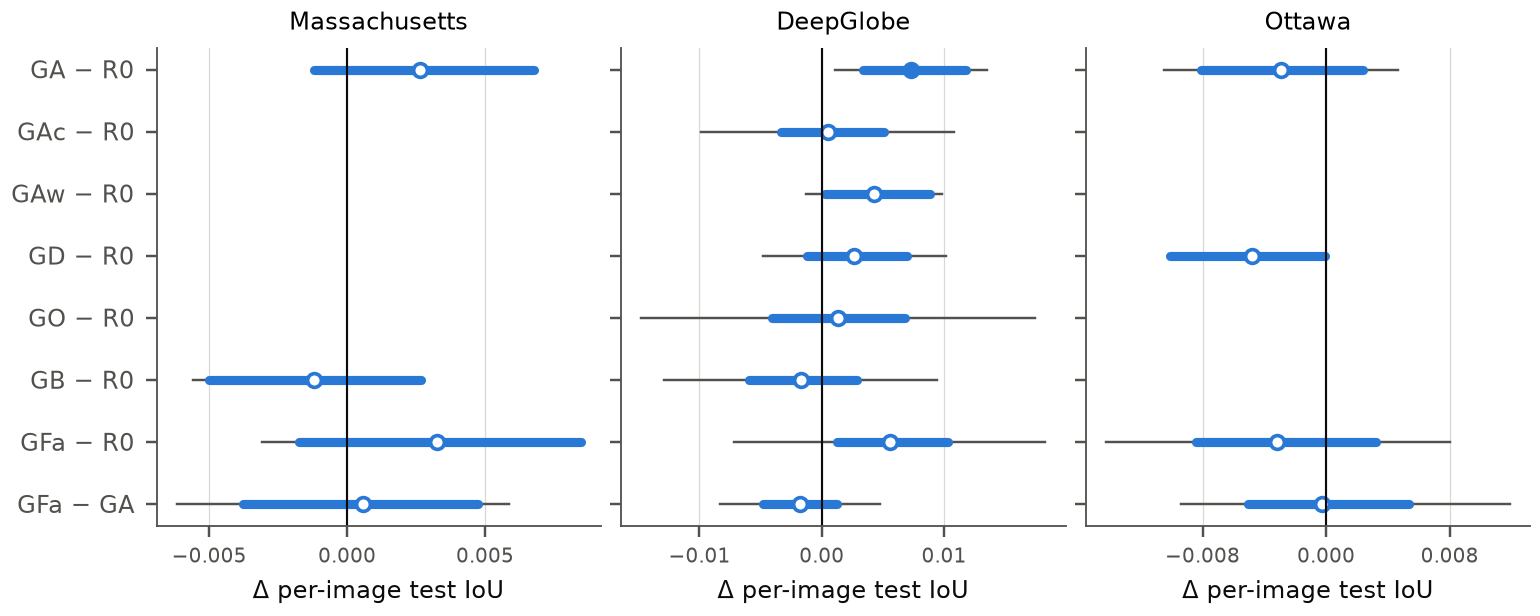
\includegraphics[width=\textwidth]{figures/forest.png}
\caption{Differences in per-image test IoU. Thick bar: two-level bootstrap 95\% CI; thin line:
seed-paired $t$ 95\% CI; filled marker: ``difference'' under the decision rule, hollow: not. Only
GA $-$ R0 on DeepGlobe meets the rule.}
\label{fig:forest}
\end{figure}

\subsection{Attribution of GA's DeepGlobe gain}
GAc $-$ R0 $+0.0005$ (no difference), GAw $-$ R0 $+0.0043$ (inconclusive: bootstrap
$[+0.0002,+0.0088]$, $t$ $[-0.0013,+0.0098]$); GA $-$ GAc $+0.0068$ and GA $-$ GAw $+0.0030$
(both differences). By the reading rule fixed in the geo2 plan, neither term alone carries the gain:
it needs both, with width contributing most (pooled 0.6849 vs.\ GA 0.6858 vs.\ R0 0.6771).

\subsection{Prior geometric targets}
On DeepGlobe GA beats DDT targets: GA $-$ GD $+0.0046$ (bootstrap $[+0.0021,+0.0072]$, $t$
$[+0.0025,+0.0068]$; per seed $+0.0055,+0.0045,+0.0038$). GD $-$ R0 $+0.0027$ and GO $-$ R0 $+0.0014$:
no detected difference. GAw $-$ GD $+0.0016$: no detected difference --- the width encoding alone is
not distinguishable from DDT's; the edge over DDT needs the centre term. On Ottawa GD $-$ R0 $-0.0048$
(inconclusive, R0 ahead).

\subsection{Geometry feedback and its selection}
Selection on validation IoU (seed 0, threshold-selected): GFa 0.6501 / 0.6879 / 0.9006 (mean 0.7462),
GFb 0.6498 / 0.6890 / 0.8986 (mean 0.7458) on Massachusetts / DeepGlobe / Ottawa: GFa selected by
0.0004. Confirmation (seeds 0--2): GFa $-$ R0 $+0.0032$ / $+0.0056$ (inconclusive) / $-0.0032$; GFa
$-$ GA $+0.0006$ / $-0.0017$ / $-0.0002$, no detected difference anywhere. On Ottawa GFa recovers part
of GA's APLS loss (0.864 vs.\ 0.839; R0 0.883), a secondary observation on six scenes.

\subsection{Error analysis}
\label{sec:errors}
Error pixels at each run's threshold, split into missed road within 2 px of the label edge (FN edge),
missed road deeper inside (FN interior), false road within 2 px of a labelled road (FP near) and
farther away (FP far); recall by label width. Means over seeds 0--2.

\begin{figure}[H]
\centering
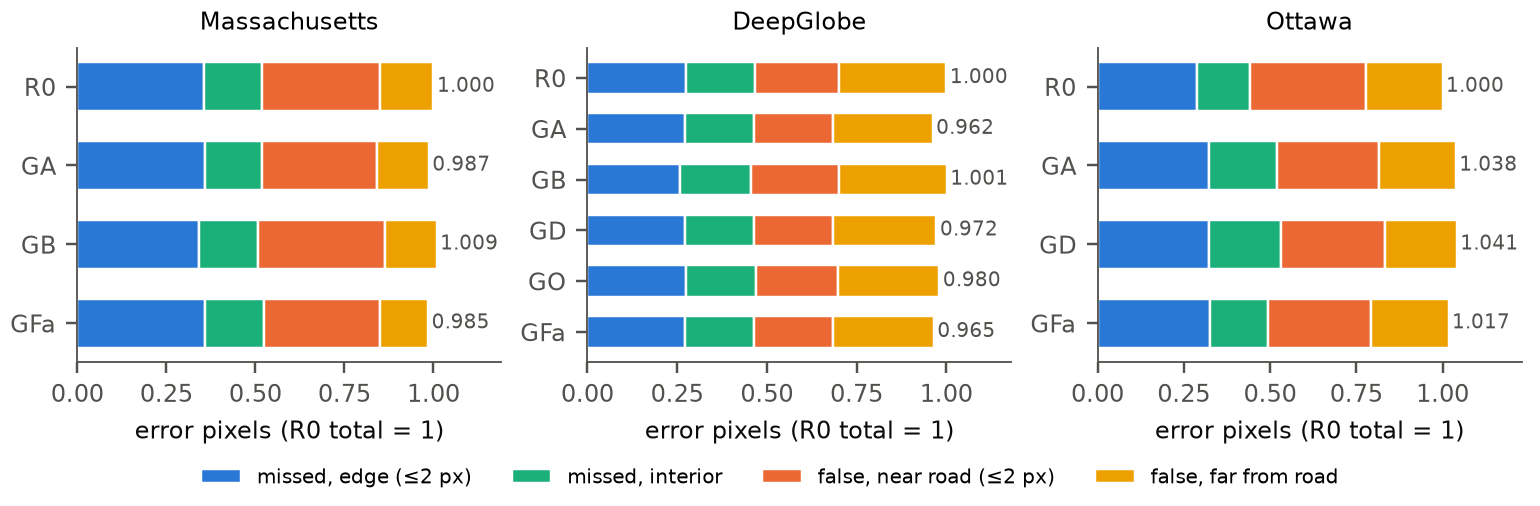
\includegraphics[width=\textwidth]{figures/errors.png}
\caption{Error composition relative to R0's total (=1). On DeepGlobe GA, GD and GFa remove false
positives (orange, yellow); on Ottawa the geometric models add missed-road errors.}
\label{fig:errors}
\end{figure}

\begin{table}[H]
\centering
\caption{Share of error pixels by type and recall by label width (px at the dataset's resolution).}
\scriptsize
\begin{tabular}{@{}lrrrrrrrrr@{}}
\toprule
 & \multicolumn{4}{c}{share of errors (\%)} & \multicolumn{5}{c}{recall by label width (px)} \\
\cmidrule(lr){2-5}\cmidrule(l){6-10}
Model & FN edge & FN int. & FP near & FP far & 1--4 & 5--6 & 7--8 & 9--12 & 13--20 \\
\midrule
\multicolumn{10}{@{}l}{\textbf{Massachusetts}} \\
R0 & 35.7 & 16.2 & 33.2 & 14.9 & 0.571 & 0.789 & 0.793 & 0.741 & 0.468 \\
GA & 36.3 & 16.2 & 32.8 & 14.6 & 0.575 & 0.789 & 0.793 & 0.751 & 0.483 \\
GB & 34.0 & 16.4 & 35.3 & 14.3 & 0.560 & 0.791 & 0.808 & 0.722 & 0.453 \\
GFa & 36.5 & 16.6 & 33.1 & 13.8 & 0.568 & 0.786 & 0.795 & 0.760 & 0.481 \\
\midrule
\multicolumn{10}{@{}l}{\textbf{DeepGlobe}} \\
R0 & 27.4 & 19.4 & 23.4 & 29.8 & 0.555 & 0.689 & 0.775 & 0.826 & 0.849 \\
GA & 28.3 & 20.0 & 22.9 & 28.8 & 0.564 & 0.683 & 0.773 & 0.829 & 0.850 \\
GB & 25.8 & 19.6 & 24.5 & 30.1 & 0.559 & 0.684 & 0.776 & 0.834 & 0.858 \\
GD & 28.0 & 19.8 & 22.6 & 29.6 & 0.548 & 0.680 & 0.772 & 0.825 & 0.853 \\
GO & 28.1 & 19.7 & 23.4 & 28.8 & 0.555 & 0.689 & 0.770 & 0.824 & 0.850 \\
GFa & 28.2 & 20.0 & 22.8 & 29.0 & 0.561 & 0.681 & 0.772 & 0.829 & 0.852 \\
\midrule
\multicolumn{10}{@{}l}{\textbf{Ottawa}} \\
R0 & 28.8 & 15.4 & 33.7 & 22.2 & 0.622 & 0.547 & 0.745 & 0.923 & 0.955 \\
GA & 31.0 & 19.0 & 28.5 & 21.5 & 0.600 & 0.542 & 0.715 & 0.908 & 0.945 \\
GD & 31.1 & 20.0 & 28.8 & 20.0 & 0.541 & 0.497 & 0.720 & 0.913 & 0.943 \\
GFa & 32.2 & 16.4 & 29.4 & 22.0 & 0.605 & 0.565 & 0.743 & 0.912 & 0.948 \\
\bottomrule
\end{tabular}

\end{table}

On DeepGlobe, relative to R0, GA changes TP by $+0.1\%$, FN by $-0.6\%$, FP-near by $-6.1\%$ and
FP-far by $-7.2\%$: the gain is precision, with recall at every width unchanged. GB misses $5.8\%$ fewer
edge pixels but adds $4.6\%$ near false positives (it draws roads slightly wide). On Ottawa every
geometric model loses recall on narrow roads (width 1--8 px).

\subsection{Training curves}
\begin{figure}[H]
\centering
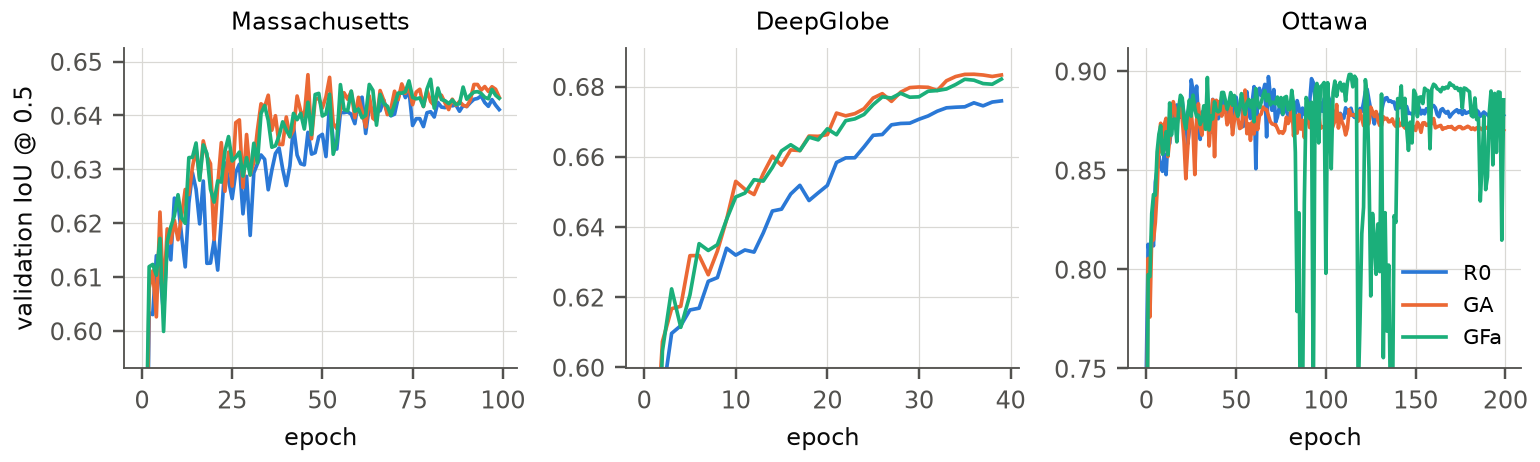
\includegraphics[width=\textwidth]{figures/curves.png}
\caption{Validation IoU at threshold 0.5 per epoch, seed 0. On DeepGlobe the geometric models lead R0
throughout training. Ottawa's validation set is two scenes, hence the noise (GFa's dips; y-axis
clipped at 0.75).}
\label{fig:curves}
\end{figure}

\subsection{Qualitative results}
\begin{figure}[H]
\centering
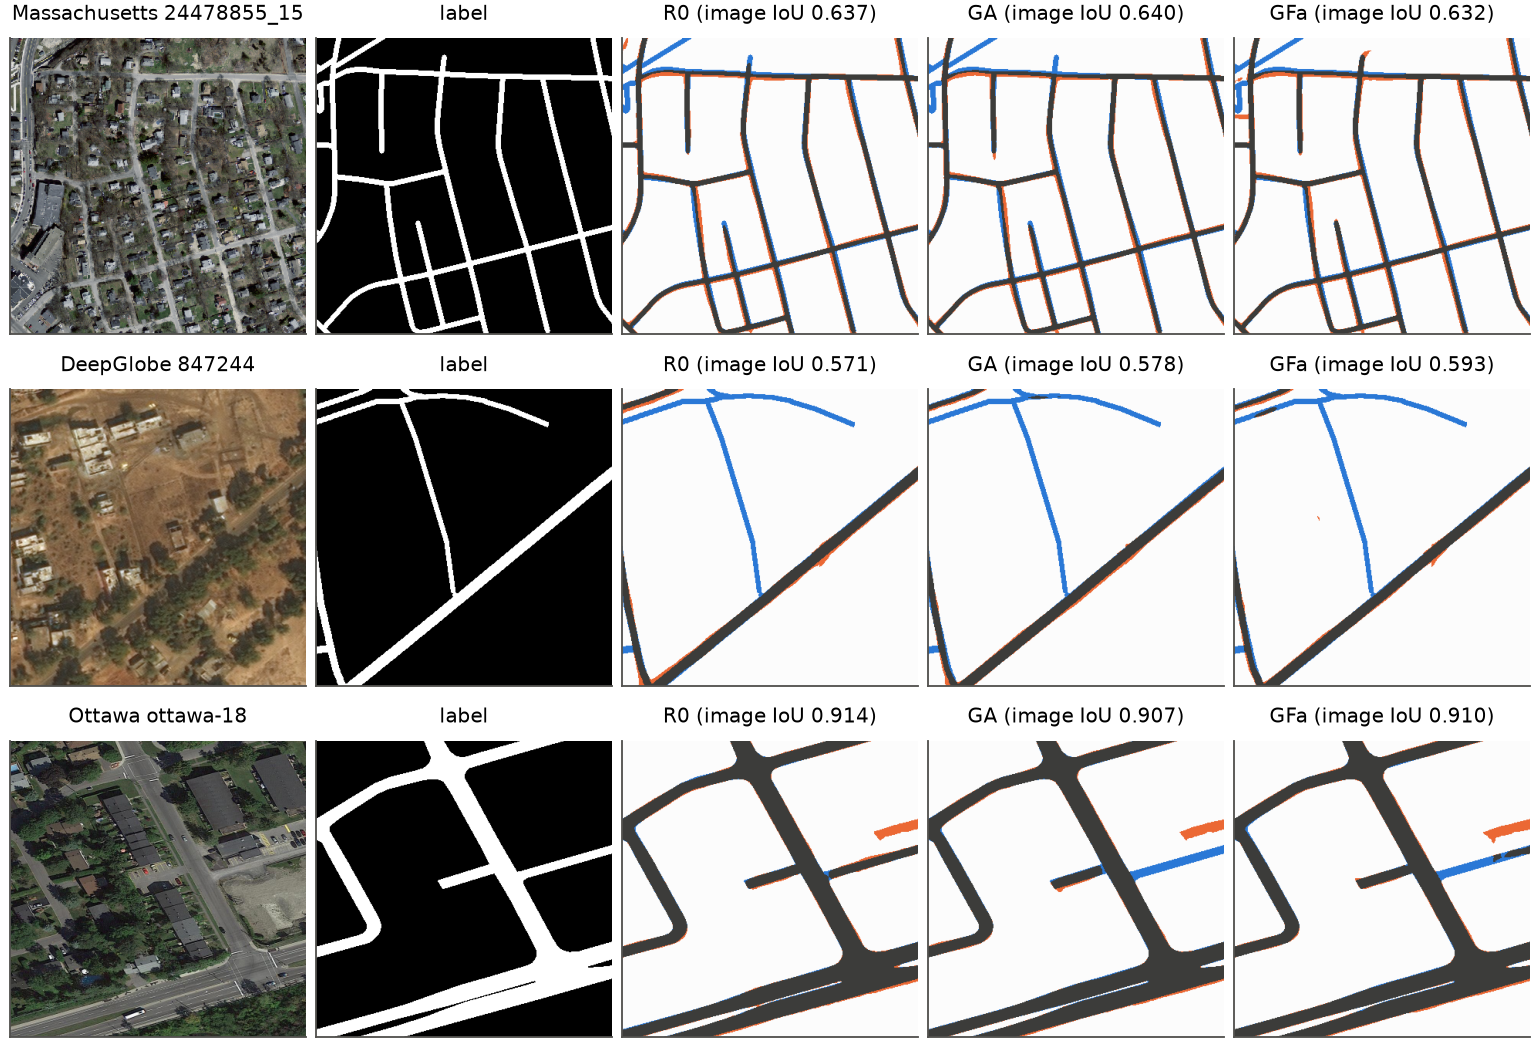
\includegraphics[width=\textwidth]{figures/qualitative.png}
\caption{One test image per dataset, chosen by rule: the image whose GA $-$ R0 difference (seed 0) is
closest to the dataset's mean difference (typical, not favourable), cropped to the $384^2$ window with
the most road. Dark grey: correct road; orange: false positive; blue: missed road.}
\label{fig:qual}
\end{figure}

%=====================================================================================
\section{Comparison with published results}
\label{sec:published}
%=====================================================================================

\begin{table}[H]
\centering
\caption{Published results and ours. Values in $[0,1]$ as printed (percentages converted).
\emph{Different splits and protocols: compare within a row group only.}}
\label{tab:published}
\scriptsize
\setlength{\tabcolsep}{3pt}
\resizebox{\textwidth}{!}{%
\begin{tabular}{@{}llccc@{}}
\toprule
Method & Protocol & Metric & Massachusetts & DeepGlobe \\
\midrule
\multicolumn{5}{@{}l}{\emph{Massachusetts official split; relaxed breakeven ($\rho=3$), as reported in \cite{zhang2018res}}} \\
Mnih-CNN \cite{mnih2013} / U-Net / ResUNet \cite{zhang2018res} & 1108/14/49 & breakeven & 0.8873 / 0.9053 / 0.9187 & --- \\
\midrule
\multicolumn{5}{@{}l}{\emph{DeepGlobe challenge server}} \\
D-LinkNet \cite{zhou2018} & val / test & road IoU & --- & 0.6466 / 0.6342 \\
NL-LinkNet \cite{wang2019nl} & val & ``mIoU'' & --- & 0.6500 \\
\midrule
\multicolumn{5}{@{}l}{\emph{DeepGlobe 4696/1530, full image \cite{batra2019}}} \\
RoadCNN / Orientation+seg.\ \cite{batra2019} & 4696/1530 & road IoU (APLS) & --- & 0.6761 / 0.6721 (0.7312) \\
\midrule
\multicolumn{5}{@{}l}{\emph{Seg-Road protocol \cite{tao2023}}} \\
D-LinkNet / CoANet / Seg-Road-l & Mass 1108/14/49; DG 4696/1530 & road IoU & 0.6145 / 0.6167 / 0.6838 & 0.5762 / 0.5911 / 0.6720 \\
\midrule
\multicolumn{5}{@{}l}{\emph{URoadNet \cite{uroadnet2024} (images resized to $512^2$)}} \\
SegFormer / URoadNet & Mass 1108/14/49; DG 4891/190/1145 & IoU & 0.6009 / 0.6761 & 0.6742 / 0.6777 \\
\midrule
\multicolumn{5}{@{}l}{\emph{DSFC-Net \cite{zhang2026dsfc}; RoadFocusNet \cite{roadfocusnet2025}}} \\
U-Net / D-LinkNet / DSFC-Net & Mass 1108/63; DG 4980/1236 & IoU & 0.6456 / 0.6443 / 0.6750 & 0.6506 / 0.6599 / 0.6868 \\
RoadFocusNet & own split & IoU & --- & 0.7083 \\
\midrule
\multicolumn{5}{@{}l}{\emph{This study: Mass 1108/14/49, no-data masked; DG 4358/933/935; stitched full images; mean of seeds}} \\
R0 / GA / GFa & as above & pooled road IoU & 0.6556 / 0.6588 / 0.6591 & 0.6771 / 0.6858 / 0.6850 \\
R0 / GA & as above & F1 & 0.7920 / 0.7943 & 0.8074 / 0.8136 \\
R0 / GA & as above & relaxed F1 ($\rho=3$) & 0.9065 / 0.9077 & 0.8978 / 0.8985 \\
R0 / GA & as above & APLS (ours) & 0.8007 / 0.8029 & 0.7755 / 0.7753 \\
\bottomrule
\end{tabular}}
\end{table}

\begin{table}[H]
\centering
\caption{Ottawa: RoadNet's road-surface results \cite{liu2019roadnet} (Table II; G = global pixel
accuracy, C = class-average accuracy, I/U = mean IoU over road and background) on the \emph{same}
test scenes 1, 16--20 at native 0.21 m, and ours at 0.42 m (mean of seeds).}
\label{tab:ottawa}
\small
\begin{tabular}{@{}lccccc@{}}
\toprule
Method & Acc.\ (G) & mIoU (I/U) & Precision & Recall & F1 \\
\midrule
FCN8s \cite{liu2019roadnet} & 0.981 & 0.919 & 0.917 & 0.932 & 0.925 \\
SegNet & 0.963 & 0.853 & 0.848 & 0.864 & 0.856 \\
U-Net & 0.973 & 0.887 & 0.899 & 0.885 & 0.892 \\
CasNet$_{++}$ & 0.983 & 0.929 & 0.932 & 0.936 & 0.934 \\
RoadNet$_{++}$ (best) & 0.985 & 0.934 & 0.936 & 0.942 & 0.939 \\
\midrule
R0 (ours, 5 seeds) & 0.984 & 0.934 & 0.933 & 0.947 & 0.940 \\
GA (ours, 5 seeds) & 0.984 & 0.932 & 0.936 & 0.940 & 0.938 \\
GFa (ours, 3 seeds) & 0.984 & 0.933 & 0.937 & 0.940 & 0.938 \\
\bottomrule
\end{tabular}
\end{table}

\paragraph{Reading the comparison.} Every paper uses its own split and protocol; only rows inside one
group are like-for-like. The same architecture (D-LinkNet) is reported at 0.576--0.666 road IoU on
DeepGlobe depending on protocol --- a spread larger than every architectural gain claimed in the
table. Our R0 is level with the strongest DeepGlobe reports under other protocols (0.672--0.687) and,
on the Ottawa test scenes, with RoadNet's best model (mIoU 0.934 vs.\ 0.934, F1 0.940 vs.\ 0.939),
although we evaluate at half resolution. Massachusetts numbers are lower than published ones partly
because we exclude no-data pixels and score stitched full images. Seg-Road's printed F1 (0.9143 with
road IoU 0.672) is inconsistent with $\IoU = F_1/(2-F_1)$, so only its road IoU is quoted.

%=====================================================================================
\section{Discussion}
%=====================================================================================

\paragraph{What helped, and why there.} The only confirmed gain is GA on DeepGlobe, made of fewer
false positives far from and near roads. DeepGlobe's scenes are rural and peri-urban with many
road-like structures (field boundaries, tracks, dry riverbeds); a width target forces the network to
commit to a plausible cross-section, which plausibly suppresses road-like texture without a coherent
width. This is an interpretation, not a tested mechanism.

\paragraph{Why it does not transfer.} On Massachusetts the labels have a constant width, so a width
target carries little information. On Ottawa the labels are precise surfaces, IoU is near 0.88 and
precision near 0.93; there is little false-positive mass to remove, and the geometric models lose
recall on narrow roads. Ottawa's six test scenes also limit power.

\paragraph{Representation vs.\ supervision.} Drawing the mask from geometry (GB) --- the analogue of
DDT's reconstruction --- did not help on either dataset and was worse than GA; DDT reported large gains
from its refinement on CT. Feeding the geometry back (GF) did not add to GA. On these data the
geometric information helps, when it helps, as a training signal, not as an output representation.

\paragraph{Against prior targets.} On DeepGlobe GA beats DDT's targets; GD and GO do not beat R0. The
advantage over DDT needs the centre-line term, since the width encoding alone (GAw) is level with GD.

%=====================================================================================
\section{Limitations}
%=====================================================================================
\begin{itemize}
  \item One confirmed positive result, on one dataset; the effect is about $+0.7$ IoU points per image.
  \item 3 seeds on DeepGlobe (5 on Massachusetts/Ottawa for R0, GA, GD); the bootstrap can be
        anti-conservative; Ottawa has 6 test scenes.
  \item Loss weights (1, 1), radii, crop counts and the recipe were not tuned; one backbone.
  \item The target design changed twice after inspecting \emph{training} masks (never val/test).
  \item The DeepGlobe confirmatory test was registered after the Massachusetts result was seen.
  \item GD and GO reuse our model and recipe, not their papers' architectures (Batra's stacked
        hourglass and refinement; DDT's 3-D networks and post-hoc refinement).
  \item Massachusetts scores exclude a custom no-data mask; DeepGlobe uses our own random split from a
        mirror; Ottawa is used at half resolution with one test scene containing 1.45\% black pixels.
  \item bf16 and non-deterministic kernels: reruns are statistically, not bitwise, reproducible.
  \item APLS is our implementation (8 px snapping, zero on miss) and not comparable with others'.
  \item CHN6-CUG was not evaluated (download behind a request form).
\end{itemize}

%=====================================================================================
\section{Reproducibility}
%=====================================================================================
{\sloppy
Repository \texttt{/scratch/hk4488/roadseg} (GitHub \texttt{HarshithKoriRaj/roadseg}, private).
Branches: \texttt{feat/geo-targets} $\to$ \texttt{feat/geo2-attribution} $\to$
\texttt{feat/geo3-baselines} $\to$ \texttt{feat/ott-dataset} $\to$ \texttt{feat/gf-feedback}. Spec:
\texttt{docs/superpowers/specs/2026-10-14-geometric-targets-design.md}; ledger (every ruling, job id and
result): \texttt{docs/superpowers/ledgers/2026-10-14-geometric-targets-ledger.md}. Every run directory
records its resolved configuration, seed, code commit, library and CUDA versions, the pretrained-weight
hash, the split sizes, the training history, the selected threshold, per-image test scores and test
probability maps. This report's numbers and figures are produced by
\texttt{scripts/analysis/report\_paper2.py} from those files.\par}

\begin{table}[H]
\centering
\caption{Campaigns (SLURM array and aggregation jobs; code snapshot).}
\small
\resizebox{\textwidth}{!}{%
\begin{tabular}{@{}llrll@{}}
\toprule
Campaign & Content & Runs & Array / aggregate & Snapshot \\
\midrule
geo & GA, GB $\times$ Mass, DG $\times$ 3 seeds & 12 & 19841566 / 19841568 & 862387b \\
geo2 & R0, GA seeds 3--4 (Mass); GAc, GAw (DG) & 10 & 20012726 / 20012727 & a6cc48b \\
geo3 & GD, GO (DG) & 6 & 20079336 / 20079337 & ba1e8e9 \\
ott & R0, GA, GD $\times$ 5 seeds (Ottawa) & 15 & 20200093 / 20200094 & 8cb06c4 \\
gfsel & GFa, GFb seed 0 $\times$ 3 datasets & 6 & 20253709 / --- & c430651 \\
gfconf\_a & GFa seeds 1--2 $\times$ 3 datasets & 6 & 20281436 / 20281440 & c430651 \\
\midrule
total & & 55 & \multicolumn{2}{l}{$\approx$220 GPU-h (paper 1: 36 runs, $\approx$170 GPU-h)} \\
\bottomrule
\end{tabular}}
\end{table}

\appendix
\section{Paper-1 models in the same table}
R1 (Haar DWT at the input with an exact, function-preserving stem), R2 (learned Haar-basis pooling and
unpooling), R3 (R2 + clDice), U-Net from scratch and D-LinkNet were trained with the identical
pipeline in paper 1 and appear in Table~\ref{tab:all} with $\dagger$. Paper 1's pre-registered result:
R1 $-$ R0 $+0.0004$ (Massachusetts) and $+0.0017$ (DeepGlobe), no detected difference.

%=====================================================================================
\begin{thebibliography}{99}\small
\bibitem{mnih2010} V.~Mnih and G.~E.~Hinton. Learning to detect roads in high-resolution aerial images. ECCV, 2010.
\bibitem{mnih2013} V.~Mnih. \emph{Machine Learning for Aerial Image Labeling}. PhD thesis, University of Toronto, 2013.
\bibitem{long2015} J.~Long, E.~Shelhamer, T.~Darrell. Fully convolutional networks for semantic segmentation. CVPR, 2015.
\bibitem{ronneberger2015} O.~Ronneberger, P.~Fischer, T.~Brox. U-Net: convolutional networks for biomedical image segmentation. MICCAI, 2015.
\bibitem{zhang2018res} Z.~Zhang, Q.~Liu, Y.~Wang. Road extraction by deep residual U-Net. IEEE GRSL 15(5):749--753, 2018.
\bibitem{demir2018} I.~Demir et al. DeepGlobe 2018: a challenge to parse the Earth through satellite images. CVPR Workshops, 2018.
\bibitem{zhou2018} L.~Zhou, C.~Zhang, M.~Wu. D-LinkNet: LinkNet with pretrained encoder and dilated convolution for high resolution satellite imagery road extraction. CVPR Workshops, 2018.
\bibitem{wang2019nl} Y.~Wang, J.~Seo, T.~Jeon. NL-LinkNet: toward lighter but more accurate road extraction with non-local operations. arXiv:1908.08223, 2019.
\bibitem{xie2017} S.~Xie, R.~Girshick, P.~Doll\'ar, Z.~Tu, K.~He. Aggregated residual transformations for deep neural networks. CVPR, 2017.
\bibitem{xie2021segformer} E.~Xie et al. SegFormer: simple and efficient design for semantic segmentation with transformers. NeurIPS, 2021.
\bibitem{tao2023} J.~Tao et al. Seg-Road: a segmentation network for road extraction based on transformer and CNN with connectivity structures. Remote Sensing 15(6):1602, 2023.
\bibitem{uroadnet2024} URoadNet: dual sparse attentive U-Net for multiscale road network extraction. arXiv:2412.17573, 2024.
\bibitem{zhang2026dsfc} Z.~Zhang et al. DSFC-Net: a dual-encoder spatial and frequency co-awareness network for rural road extraction. arXiv:2602.01278, 2026.
\bibitem{roadfocusnet2025} RoadFocusNet: road extraction from remote sensing imagery using focused transformer and focused masked image modeling. International Journal of Digital Earth, 2025.
\bibitem{mattyus2017} G.~M\'attyus, W.~Luo, R.~Urtasun. DeepRoadMapper: extracting road topology from aerial images. ICCV, 2017.
\bibitem{mosinska2018} A.~Mosinska, P.~M\'arquez-Neila, M.~Kozi\'nski, P.~Fua. Beyond the pixel-wise loss for topology-aware delineation. CVPR, 2018.
\bibitem{shit2021} S.~Shit et al. clDice --- a novel topology-preserving loss function for tubular structure segmentation. CVPR, 2021.
\bibitem{mei2021} J.~Mei, R.-J.~Li, W.~Gao, M.-M.~Cheng. CoANet: connectivity attention network for road extraction from satellite imagery. IEEE TIP 30:8540--8552, 2021.
\bibitem{vanetten2018} A.~Van~Etten, D.~Lindenbaum, T.~M.~Bacastow. SpaceNet: a remote sensing dataset and challenge series. arXiv:1807.01232, 2018.
\bibitem{bastani2018} F.~Bastani et al. RoadTracer: automatic extraction of road networks from aerial images. CVPR, 2018.
\bibitem{he2020sat2graph} S.~He et al. Sat2Graph: road graph extraction through graph-tensor encoding. ECCV, 2020.
\bibitem{hetang2024} C.~Hetang et al. Segment anything model for road network graph extraction. CVPR Workshops, 2024.
\bibitem{wang2020ddt} Y.~Wang, X.~Wei, F.~Liu, J.~Chen, Y.~Zhou, W.~Shen, E.~K.~Fishman, A.~L.~Yuille. Deep distance transform for tubular structure segmentation in CT scans. CVPR, 2020 (arXiv:1912.03383).
\bibitem{batra2019} A.~Batra, S.~Singh, G.~Pang, S.~Basu, C.~V.~Jawahar, M.~Paluri. Improved road connectivity by joint learning of orientation and segmentation. CVPR, 2019.
\bibitem{liu2019roadnet} Y.~Liu et al. RoadNet: learning to comprehensively analyze road networks in complex urban scenes from high-resolution remotely sensed images. IEEE TGRS 57(4), 2019. Dataset: \url{https://github.com/yhlleo/RoadNet}.
\bibitem{cascade2022} Cascaded multi-task road extraction network for road surface, centerline, and edge extraction. IEEE TGRS, 2022 (IEEE Xplore 9756441).
\bibitem{wei2020width} Y.~Wei, X.~Hu, M.~Zhang, Y.~Xu. Automatic extraction of road centerlines and edge lines from aerial images via CNN-based regression. ISPRS Annals V-2-2020:925, 2020.
\bibitem{brightearth2024} BrightEarth roads: towards fully automatic road network extraction from satellite imagery. arXiv:2406.14941, 2024.
\bibitem{connectivity2023} Fine-grained extraction of road networks via joint learning of connectivity and segmentation. arXiv:2312.04744, 2023.
\bibitem{location2021} Road extraction from satellite image via auxiliary road location prediction. IEEE IGARSS / Xplore 9554086, 2021.
\bibitem{henry2020noise} C.~Henry, S.~M.~Azimi, N.~Merkle. Aerial road segmentation in the presence of topological label noise. ICPR, 2020.
\bibitem{globalroad2024} Global road extraction using a pseudo-label guided framework: from benchmark dataset to cross-region semi-supervised learning. Geo-spatial Information Science, 2024 (doi:10.1080/10095020.2024.2362760).
\bibitem{zhu2021chn6} Q.~Zhu et al. A global context-aware and batch-independent network for road extraction from VHR satellite imagery. ISPRS J.\ Photogramm.\ Remote Sens., 2021 (CHN6-CUG dataset).
\end{thebibliography}

\end{document}
